\documentclass[11pt]{article}
\usepackage{graphicx} 
\usepackage{multicol}
\usepackage{geometry}
\usepackage{amsmath}
\usepackage{booktabs}

\geometry{
    left=2cm,
    right=2cm,
    top=2cm,
    bottom=2cm
}


\title{Volume Computation of 3D Reconstructed Objects From Volumetric Data Using Binary Indexed Tree}
\author{Nguyen Le Quoc Bao \& Le Tuan Hy}
\date{8 March 2024}

\begin{document}

\maketitle

\begin{center}
\begin{minipage}{0.8\textwidth}
\setlength{\leftskip}{3.5cm} 
\setlength{\rightskip}{3.5cm}
\begin{abstract}
    In the burgeoning field of medical imaging, precise computation of 3D volume holds a significant importance for subsequent qualitative analysis of 3D reconstructed objects. Combining multivariable calculus, marching cubes algorithm, and binary indexed tree data structure, we develop a algorithm for efficient computation of intrinsic volume of any volumetric data retrieved from computed tomography (CT) or magnetic resonance (MR). We proposed the 30 configurations of volume values based on polygonal mesh generation method. Our algorithm processes the data in scan-line order to initialize the Fenwick tree simultaneously with the reconstruction algorithm, ensuring faster volume query time following users edition such as slicing or transforming object mesh. We tested the algorithm's accuracy on simple 3D objects (e.g.sphere) to complicated structures (11 cardiac components). The result deviated slightly from labelled volume and there is still space for further improvement.
\end{abstract}
\end{minipage}
\end{center}

\begin{multicols}{2} 
\section{Introduction}
This research is one pivotal component in our larger research project "Integration of Deep Learning into automatic cardiovascular dissection and reconstruction in simulated 3D space for medical practice". Therefore, this research is mostly focused on medical volumetric data, especially human cardiac CT scans. In the contemporary landscape of medical imaging, the conversion of tomographic data into precise three-dimensional (3D) models stands as a burgeoning trend of paramount importance. Since three-dimensional surfaces of anatomy offer a valuable medical tool. The 3D representation helps physicians/radiologists with better intepretation of volumetric data \cite{loren}. The evolution in 3D medical imaging necessitates robust post-processing methodologies to ensure the meticulous measurement and analysis of these intricate 3D structures with utmost accuracy and efficiency \cite{intrinsic}. Of particular significance is the quantification of various parameters within the cardiovascular system, including but not limited to the diameter, area, and volume of critical structures such as the aortic duct. These metrics serve as crucial indicators for pathologies such as hypertrophy or stenosis, which pose significant risks to patient well-being. Consequently, the accurate assessment and preoperative planning facilitated by such analyses substantially enhance the clinical efficacy and safety of surgical interventions. While existing software proficiently translates medical tomographic data into comprehensive 3D representations, the capability to perform volumetric analysis remains conspicuously absent, thereby warranting further advancements in this critical domain.

\subsection{System processing flow}
Our software system starts from the second step to the last one. The post processing in \cite{vascular} consists of many advanced functions for radiologists to control 3D objects both on computer and in vritual reality environment. \\
- Data Acquisition \\ 
- Image Processing \\
- Segmentation \\ 
- 3D Reconstruction \\ 
- Rendering \& display \\
- Post processing 

\section{Literary review}
The Marching Cubes algorithm, proposed by Lorensen in 1987, is commonly used for 3D mesh reconstruction from CT scans. However, it has limitations due to a small lookup table. To address this, Lewiner \cite{lewiner} proposed an improved version with an extended lookup table, resolving the “cracks” issue. This development requires efficient automatic post analysis, especially measuring important parameters such as volume, surface area, curvature. \cite{limb} presents a system to measure limb volumes using 3D models from an infrared depth sensor. However, this method does not leverage advanced computed imaging (CT, MR) and may be affected by environmental factors. Intrinsic volume measurement techniques directly from digital 3D images have been explored \cite{intrinsic}, but their computational complexity remains a challenge. 

\section{Methodology}
Since our main application is in medical imaging, especially cardiac volumetric data, we only focus practical experiment and analysis in this specific field. 

\subsection{Integral of surface functions}

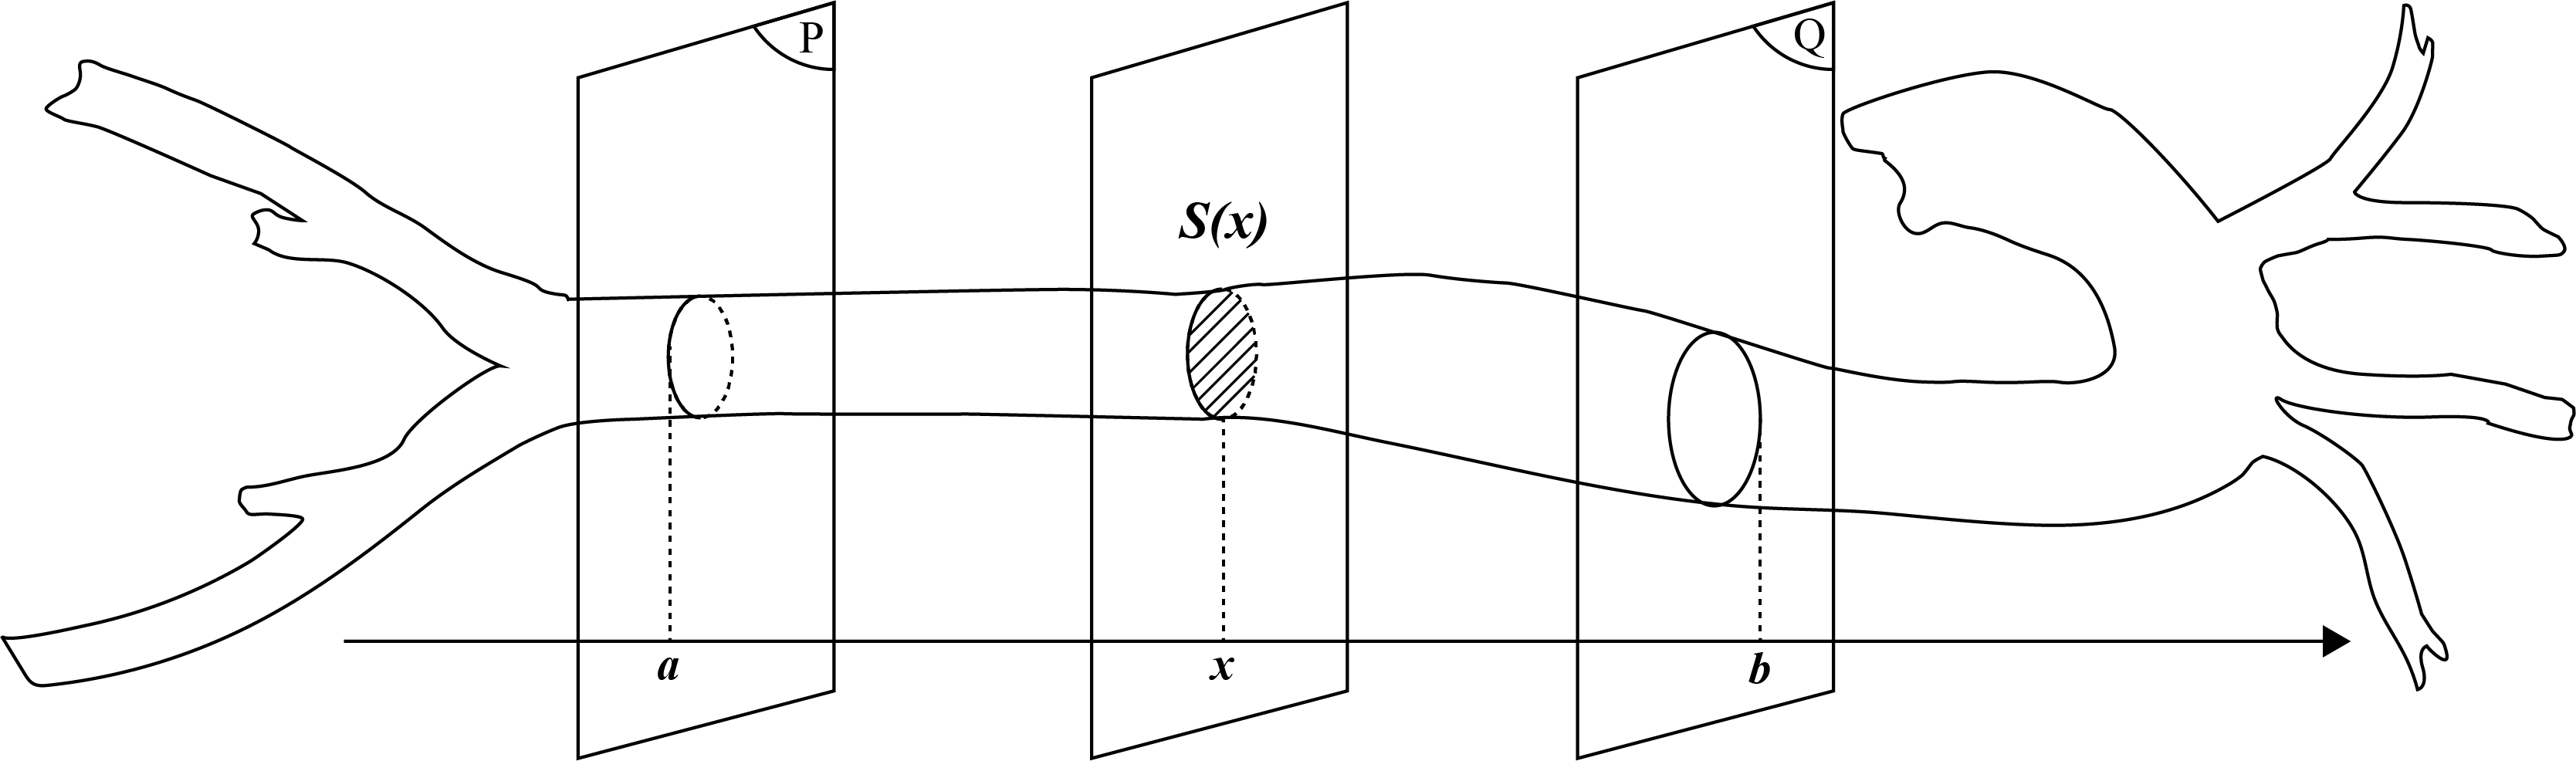
\includegraphics[width=0.48\textwidth]{Figures/Integral Surface Function.png}
\textbf{Figure 1:} Calculating the volume of the aortic duct by integrating the surface function \\

We can determine whether the arterial duct is hypertrophied by comparing its volume to standard parameters. We intersect the aorta with two planes $(P), (Q)$ using a Symmetric Ray Casting method \cite{vascular}. The limits $a,b$ on the $Ox$ axis of an object are $(x=a, x=b, a \leq b)$. A plane perpendicular to the $Ox$ axis at point $x$ and $a \leq x \leq b$ intersects the object with a cross-sectional area of $S(x)$ and the equation $S(x)$  is continuous on the interval $[a;b]$. Thus, the volume of the upper heart chamber is calculated by the following integral formula:
$$
V = \int_{a}^{b} S(x)dx
$$
For a set of $n$ slice images, we have $S_i$ as the area of the $i_{th}$ slice $(1 \leq i \leq n)$. Approximating a function $S(x)$ is not straightforward. We can use the Lagrange interpolation method. However, this approach has many limitations. Firstly, the approximation is only accurate if $n \rightarrow \infty$ to ensure accuracy. This is practically infeasible because the number of slices $n$ is usually not large enough $(300 \rightarrow 512)$ and is limited. Secondly, approximating a function is also a complex task, increasing algorithm's processing time.

\subsection{Inclusion and exclusion principle}
Double integral problem is an combination of multiple single integral problems. Initially, we divide the curved surface $z=f(x,y)$ into surfaces $S_j, S_{j+1}, \dots, S_m$ corresponding to each $y_j,  y_{j+1}, \dots, y_m$ where each surface $S_j$ with fixed $y_j$ represents a single integral problem. Finally, we sum up these surfaces $S_j$ to calculate the volume $V$: 
$$
D = \begin{cases} a \leq x \leq b \\ c \leq y \leq d \end{cases} \\
$$
$$
V =  \int_{c}^{d} \begin{pmatrix} \int_{a}^{b} f(x,y)dx \end{pmatrix} dy = \int_{c}^{d} dy \int_{a}^{b} f(x,y)dx \space
$$

With inclusion and exclusion principal, we can measure the volume of predetermined structure. For example, When calculating the volume of the aortic arch, we divide this vessel into two parts: the upper half $o_1$ and the lower half $o_2$ so the domain $D$ remains the same. The volume of the inner part will be $V_o = V_{o_1} - V_{o_2}$ :

$$
V_o = V_{o_1} - V_{o_2} \\
$$
$$
V_o = \lim_{\Delta x_i, y_j \rightarrow 0} \Sigma_{j=c}^{j=d} (\Sigma_{i=a}^{i=b} (z^{o_1}_{ij} - z^{o_2}_{ij}) \Delta x_i) \Delta y_j
$$ \\

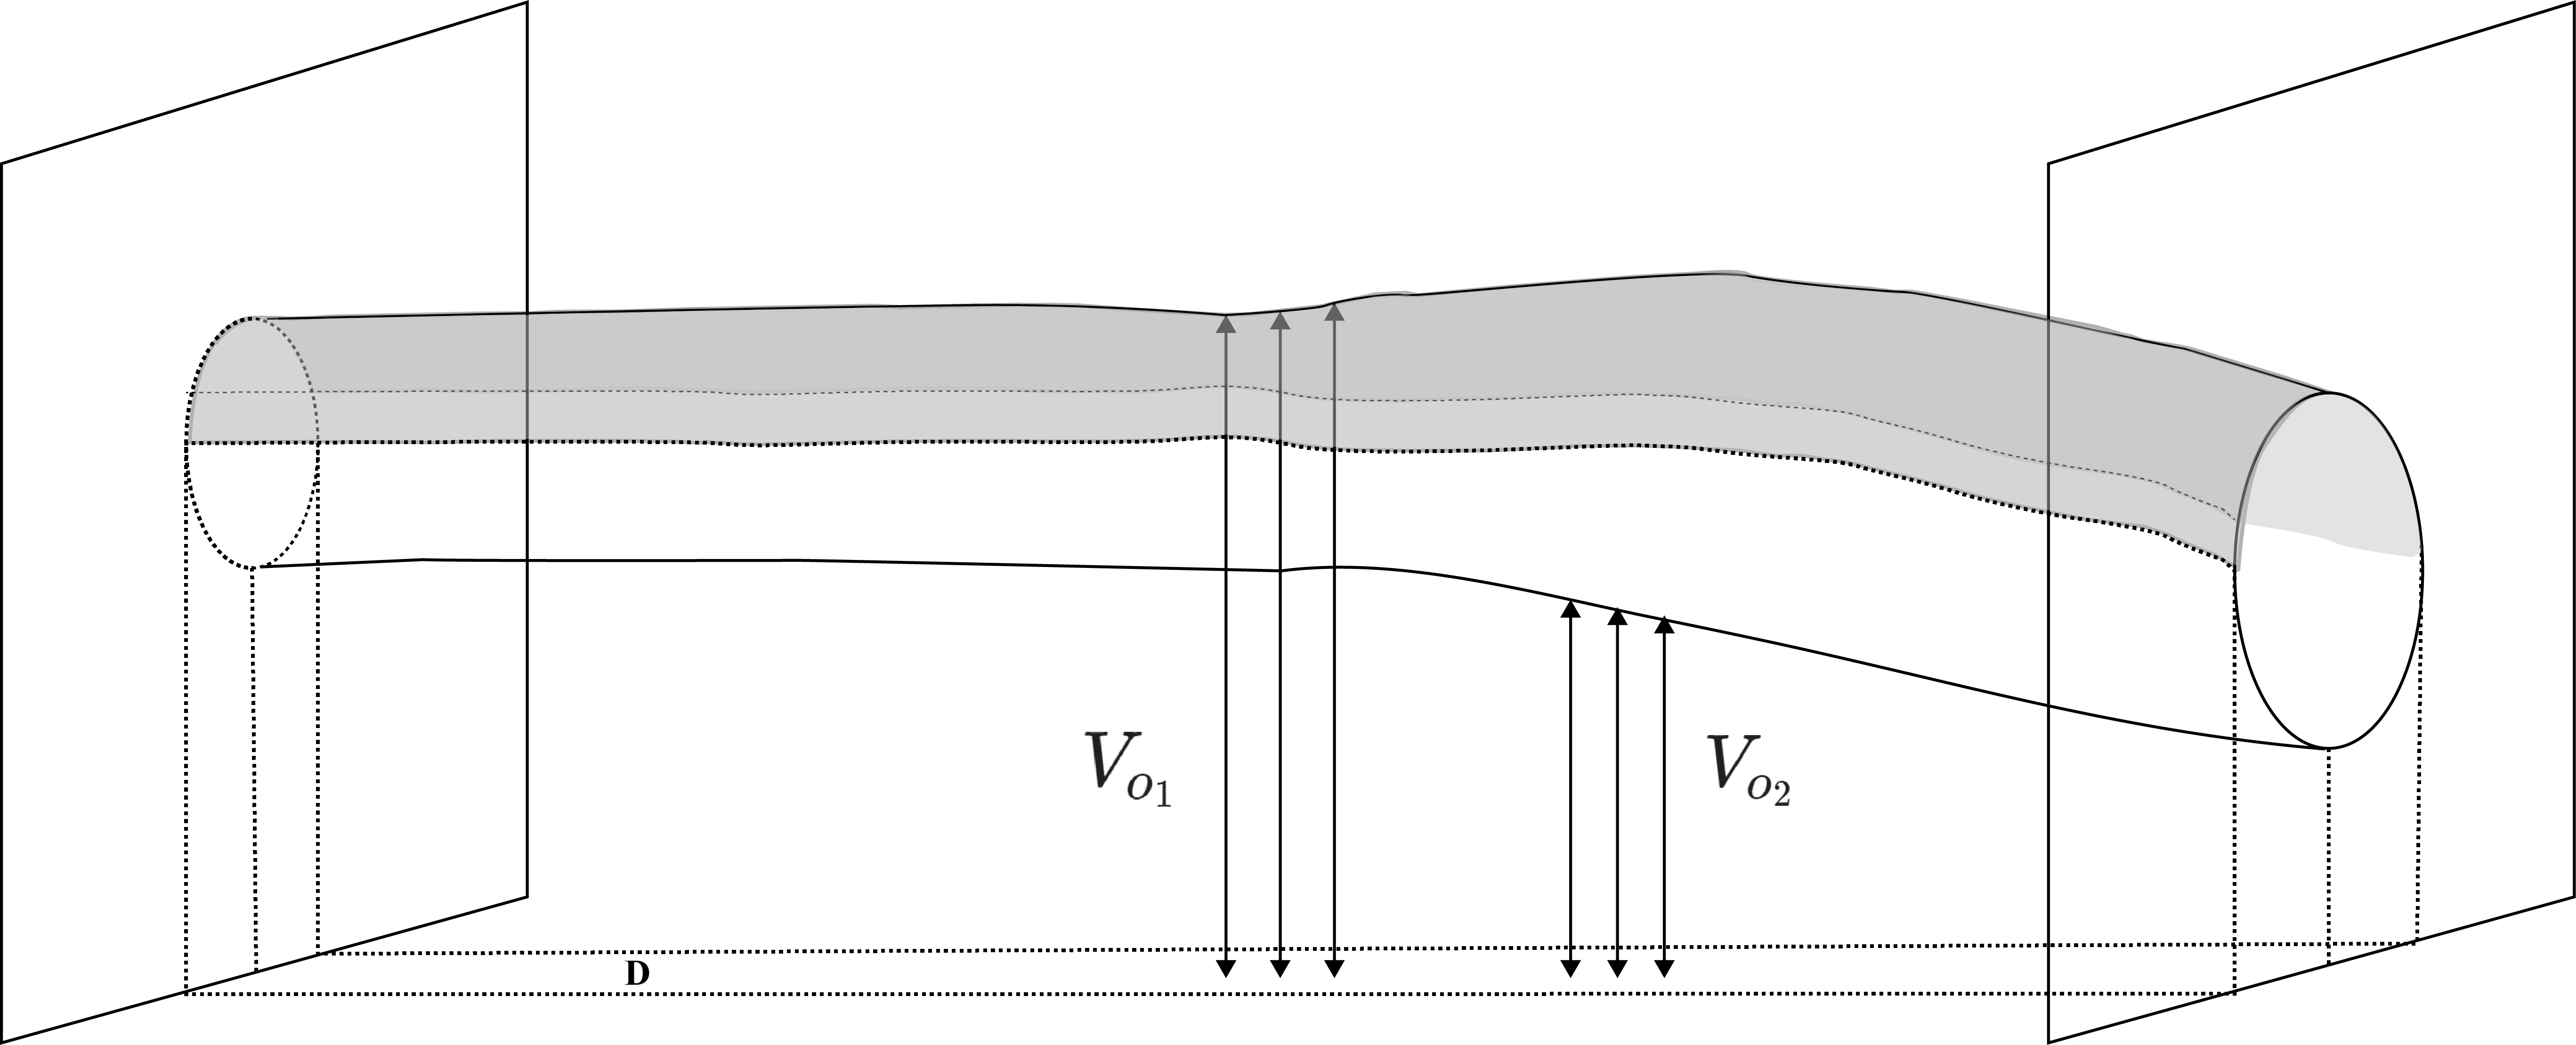
\includegraphics[width=0.45\textwidth]{Figures/Exclusion.png}
\textbf{Figure 2:} Calculating partial aortic arch volume with double integral \\

Given a list of $(x,y,z)$ vertices, the implementation of this approach computed the volume of tube structures accurately . However, we have to find a midsection to divide the object into two parts. Additionally, current software systems \cite{vascular} allows radiologists to perform surgical operations (e.g. slicing) or modifies the segmentation result leading to changes in the 3D reconstructed polygonal mesh, so algorithm must reprocess again. If denoting $Q$ as the times of slicing or updating operation is performed, the time complexity will be $O (Q \times (M \times N + S))$, where S represents the complexity of finding midsection path. This issue can be optimized with triple integral combined with binary indexed tree.

\subsection{Triple integral}
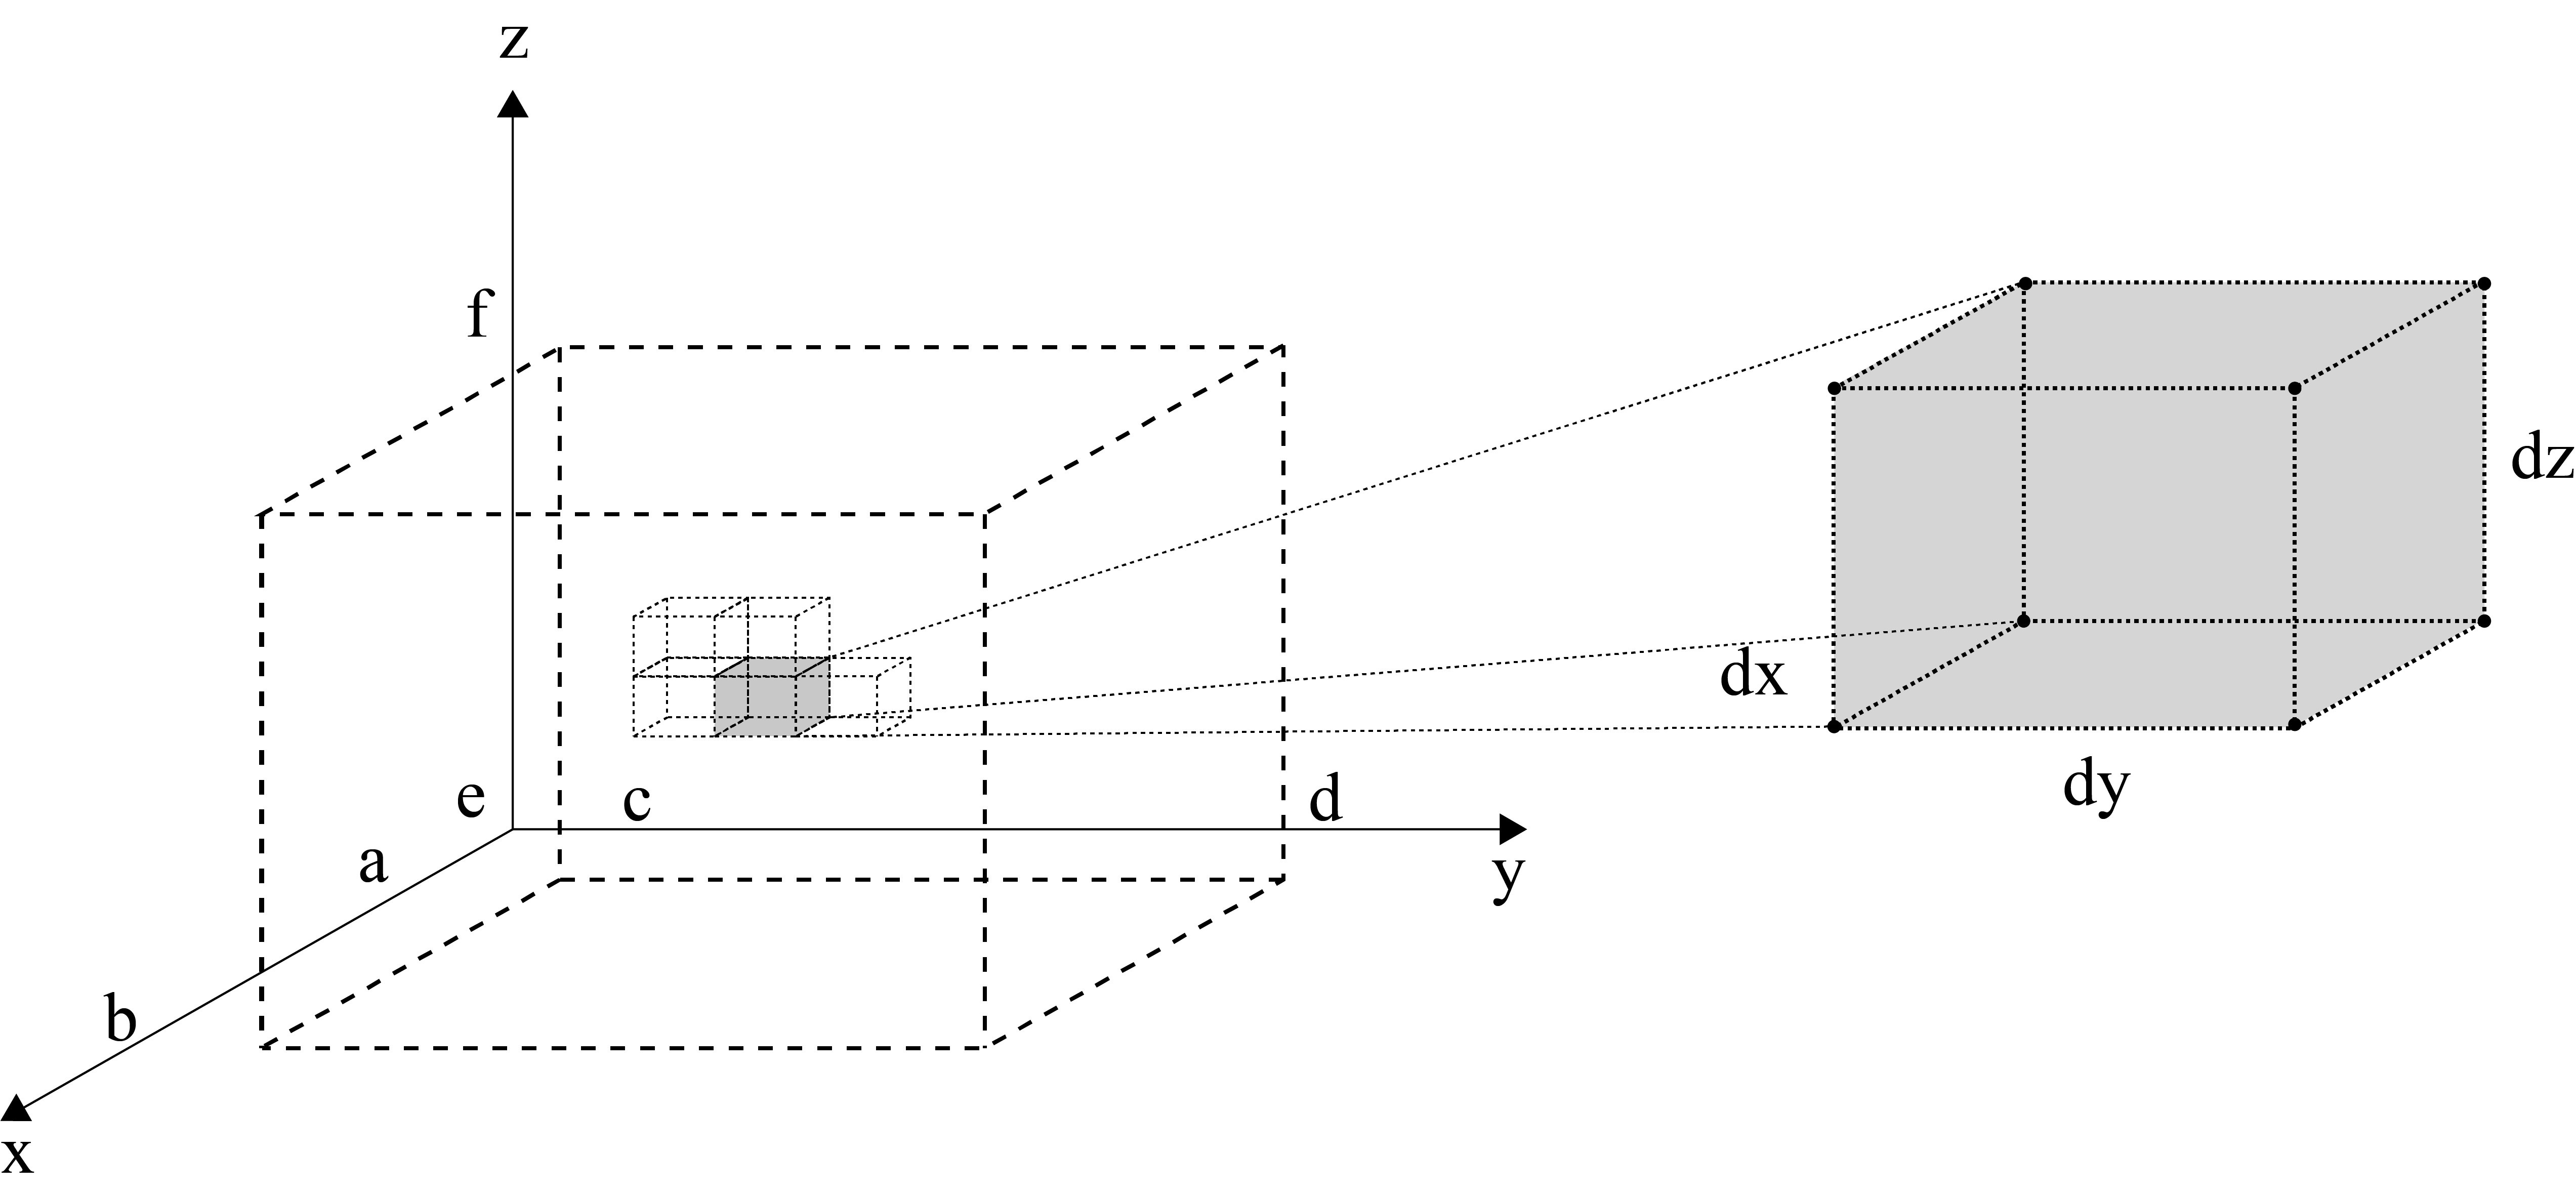
\includegraphics[width=0.45\textwidth]{Figures/Triple Integral.png}
\textbf{Figure 3:} Calculating the volume of an object with triple integration  \\

The concept of triple integration originates from dividing the object volume $O$ into n very small rectangular prisms or cubes $O_i$ with lengths, widths, and heights denoted as $dx,dy,dz$ respectively. Approximating the volume of the original object is straightforward by summing the volumes of all $O_i$ with $1 \leq i \leq n$ and as $n \rightarrow +\infty$:
$$
V = \lim_{n \rightarrow + \infty} \Sigma_{i=1}^{n} \Delta z_i \Delta y_i \Delta x_i
$$

The above formula shows that each cube is processed in three dimensional loops over $Ox, Oy, Oz$, which is comprehensively compatible with the marching algorithm. Therefore we integrate the approximation idea of triple integral into marching cubes algorithm and store the calculated data into 3D binary indexed tree.

\subsection{Volume configurations in Marching Cubes}

Marching cubes uses a divide-and-conquer approach to locate the surface in a logical cube created from eight pixels; four each from two adjacent slices \cite{loren}. In three dimensional space, the relationship between a cube and the 3D model is classified into three cases: the cube is totally inside the object, partly intersected by the surface mesh, or totally located outside the object. The surface can intersect the cube in $2^8=256$ cases since a cubes has $8$ vertices in total (this can be proved by generation method). \\

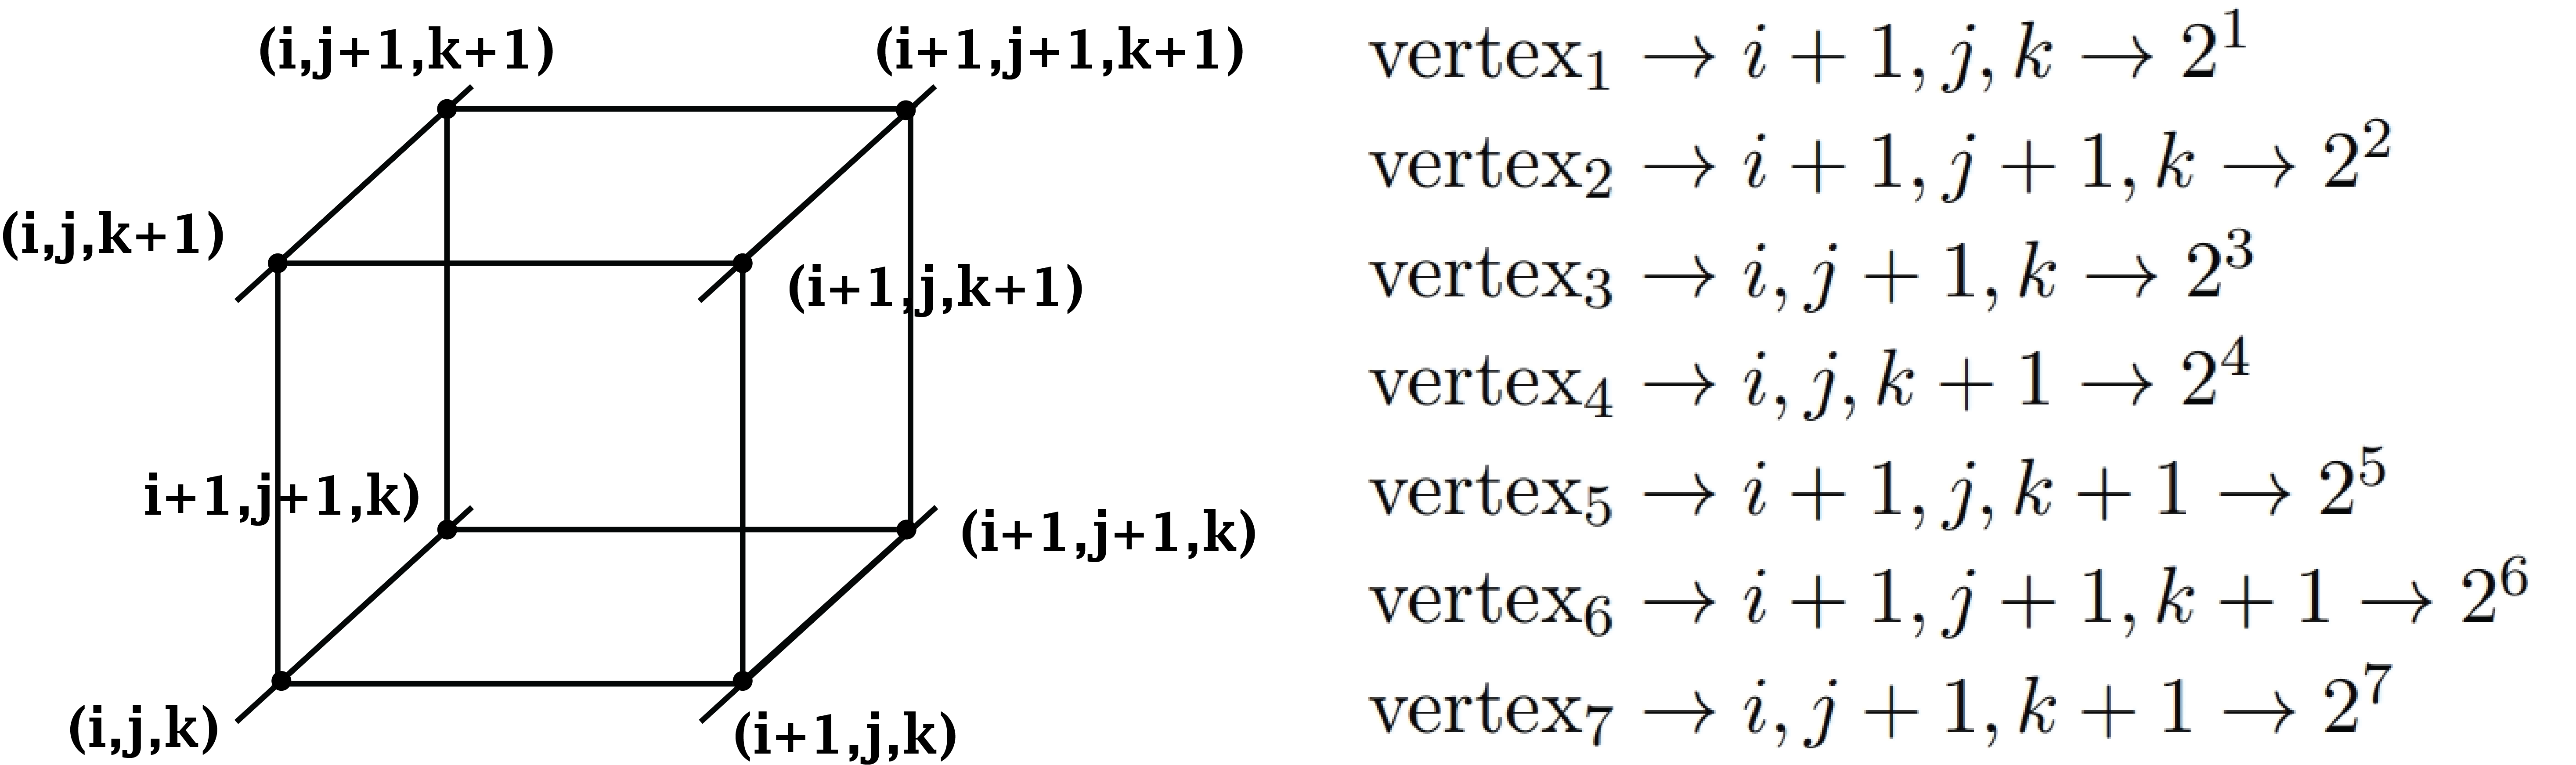
\includegraphics[width=0.46\textwidth]{Figures/Binary Vertices.png}
\textbf{Figure 4:} Vertex indexing and binary representation  \\

However, \cite{loren} reduced the problem from 256 cases to 14 patterns by utilizing symmetrical property, rotational symmetry. From original 3D array, the algorithm create the boolean 3D array with the same size speculating that a vertex is false if locates inside the model and vice versa. Therefore, the volume of the model within a cube is limited from the mesh generated to all False vertices. Although the topologically triangulated mesh is unchanged when performing rotation or symmetrical operations, the volume is changed. Specifically, the volume of case $j$ is equal to $1-V_i$ with $j$ is the reversed case of $i$. Finally, we have up to $28$ cases of volume plus $2$ cases (all vertices are either False or True), which totally is $30$ cases. The specified volume of each $30$ cases is presented in figure $4$.

The volume is each case easily calculated by dividing the 3D shape into simple shapes such as tetrahedron, prism,... The formulas are:
$$ V_{\text{tetrahedron}} = \frac{1}{3} h S_{\text{base}} $$
$$ V_{\text{prism}} = h S_{\text{base}} $$ 

With more complicated reconstructed mesh, we assigned coordinates to the cubes and use vectors operations (e.g. dot-product, cross-product). For example, given 4 points $A(x_A,y_A,z_A)$, $B(x_B,y_B,z_B)$, $C(x_C,y_C,z_C)$, $D(x_D,y_D,z_D)$, we have:
$$
V_{ABCD} = \frac{1}{6} |\Vec{AB} \times \Vec{AC}| \cdot \Vec{AD}
$$
\end{multicols}
\begin{table}[]
    \centering
    \begin{tabular}{c|c|c|c|c|c}
        \textbf{Cases} & \textbf{Calculation} & \textbf{Explanation} & \textbf{Volume} & \textbf{Reversed case} & \textbf{Reversed Volume}\\
    \midrule
        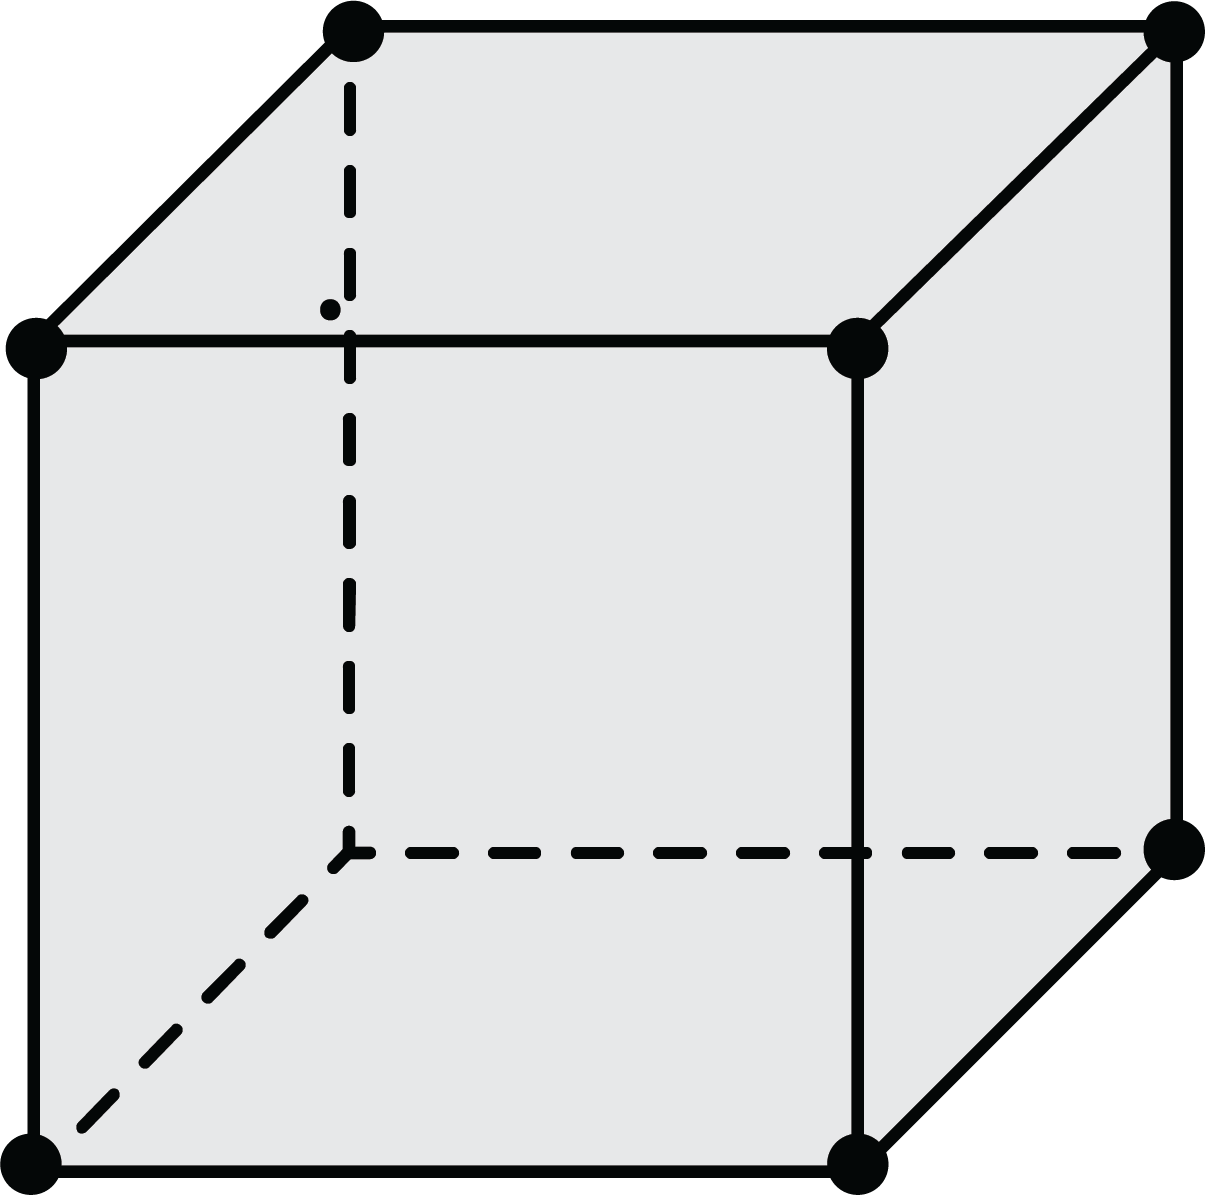
\includegraphics[width=1cm]{Figures/case 1.png} & $1 \times 1 \times 1$ & 1 cube & $1$ & 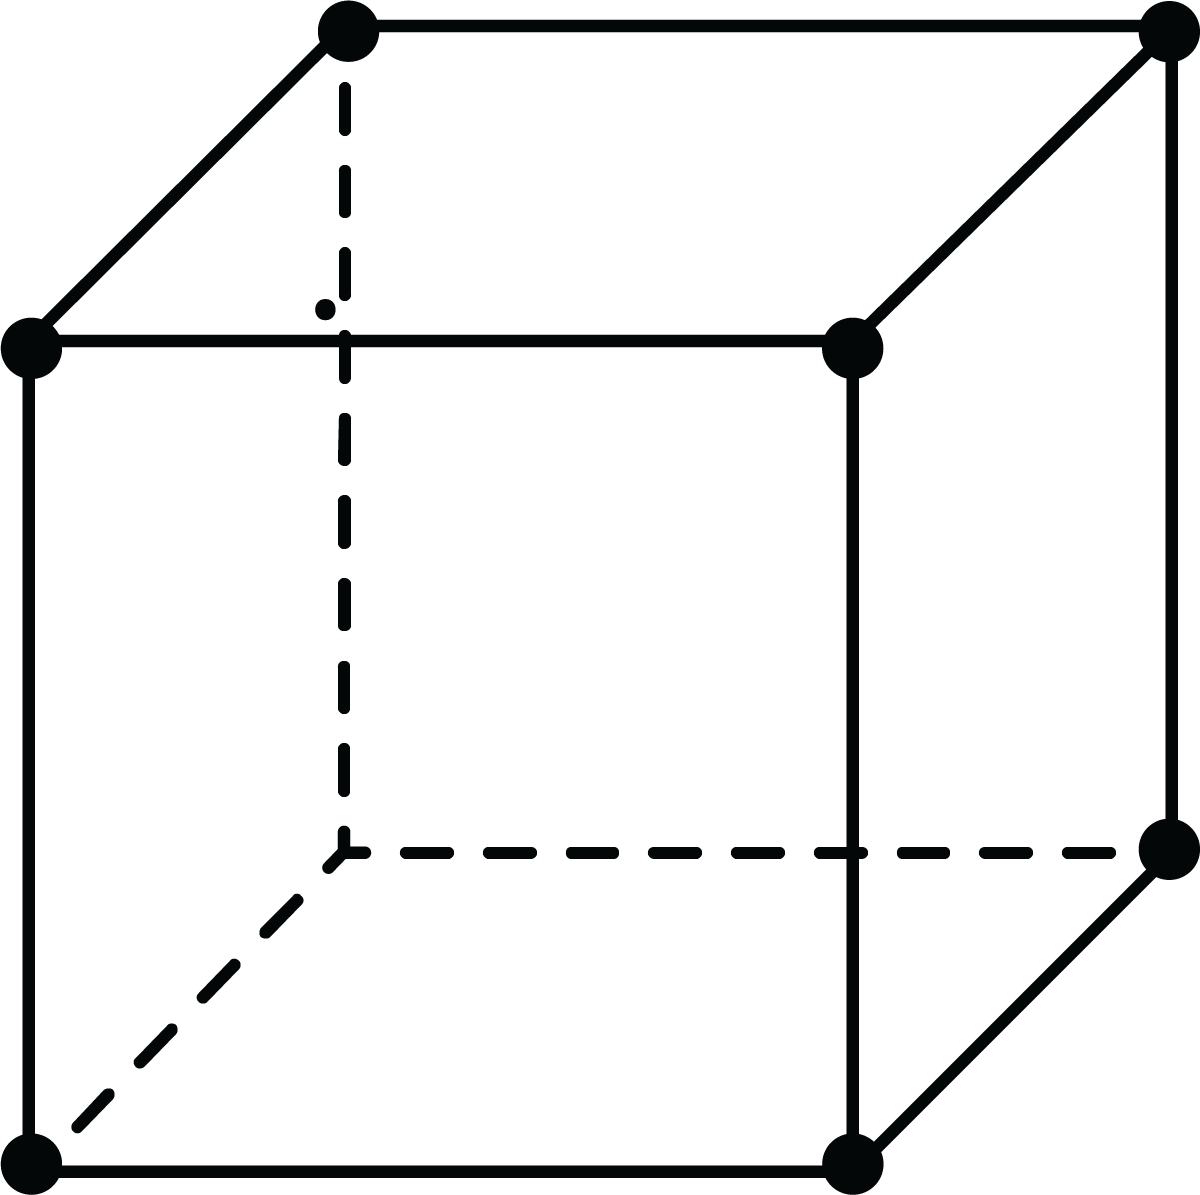
\includegraphics[width=1cm]{Figures/case 16.png} & $0$ \\
    
        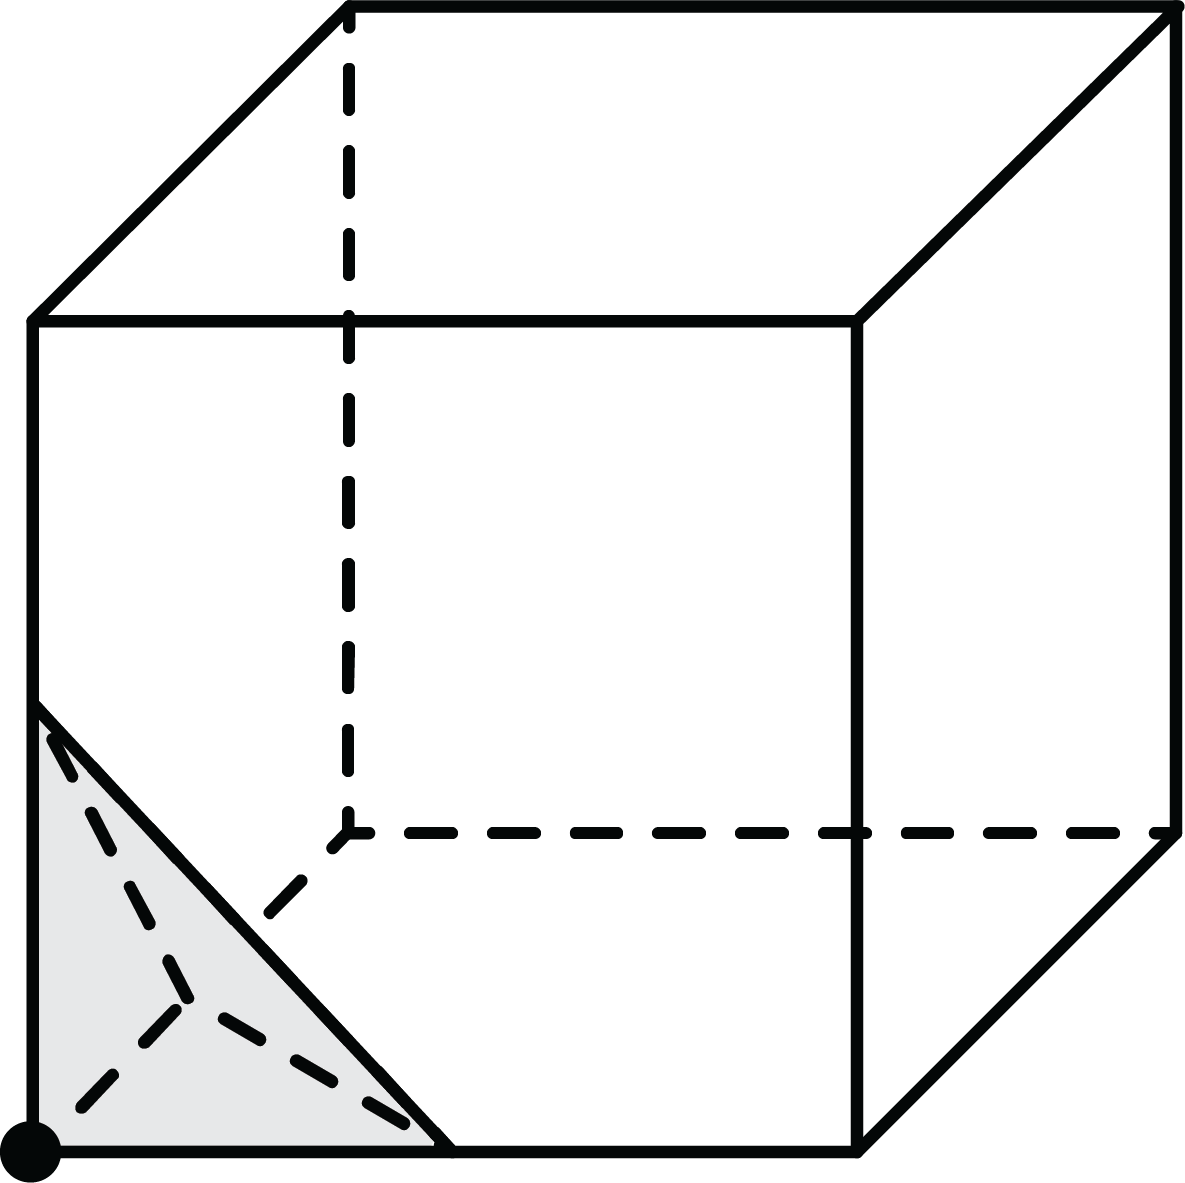
\includegraphics[width=1cm]{Figures/case 2.png} & $\frac{1}{3} \times 0.5 \times \frac{1}{2} \times 0.5^2$ & 1 tetrahedron & $\frac{1}{48}$ & 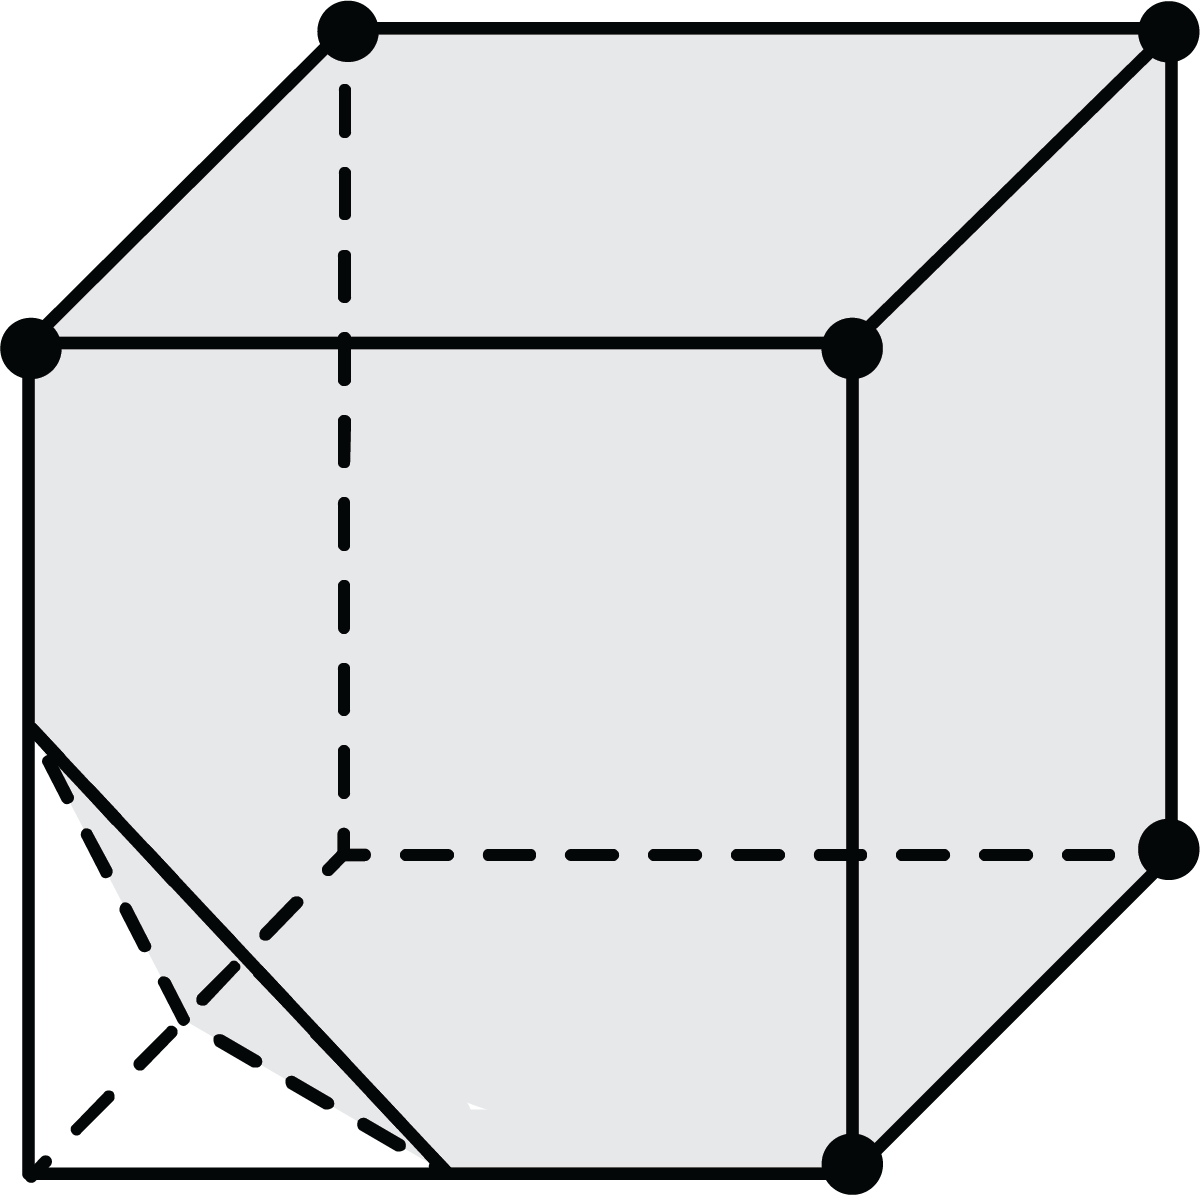
\includegraphics[width=1cm]{Figures/case 17.png} & $\frac{47}{48}$\\

        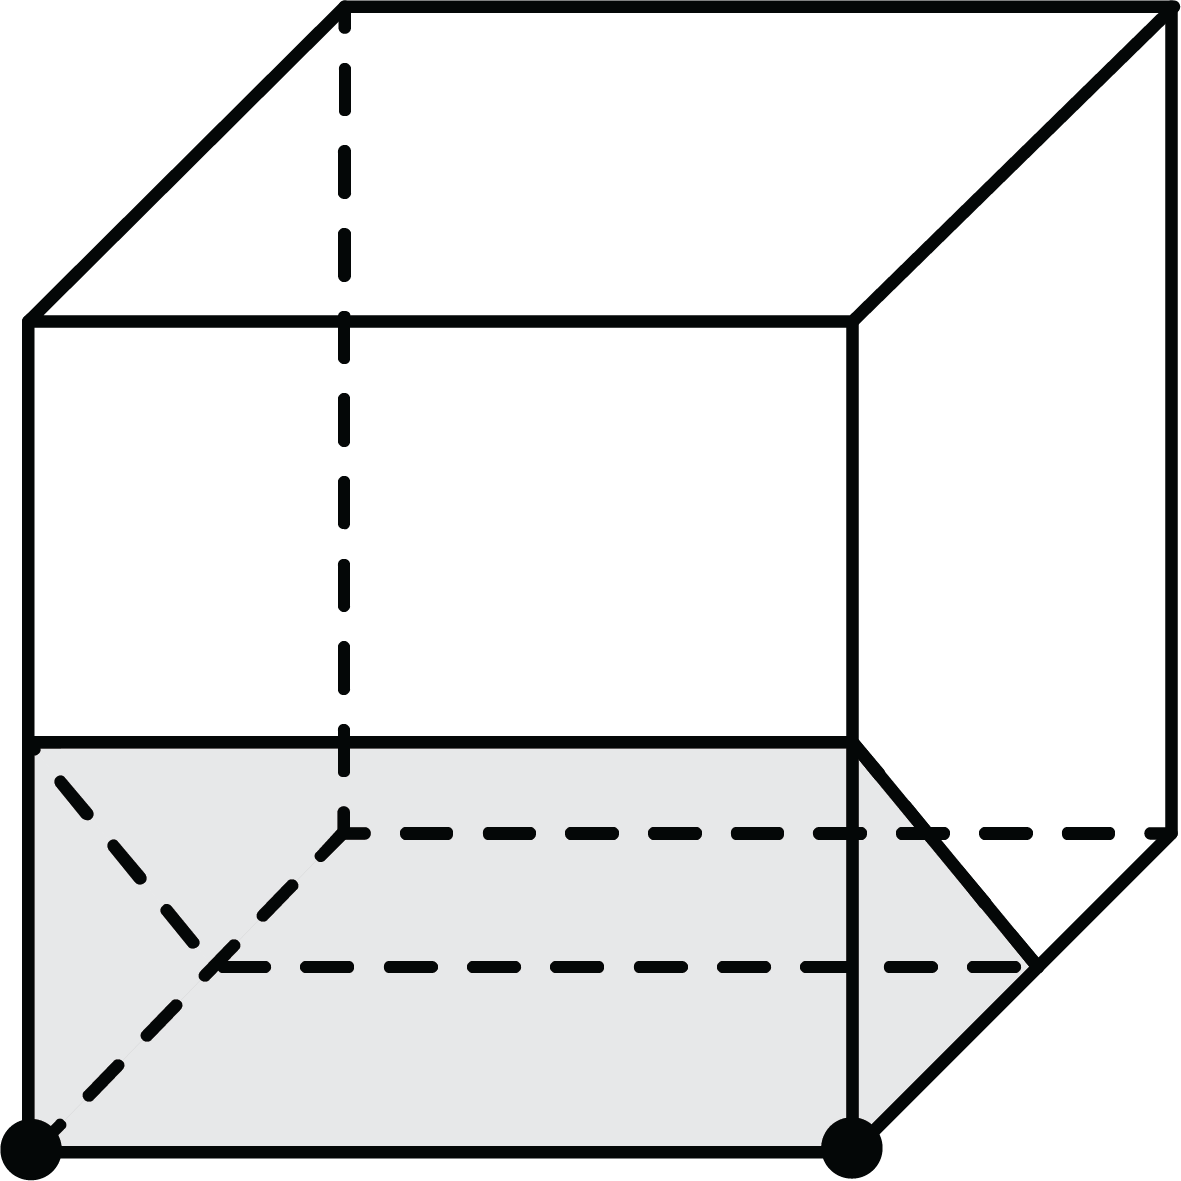
\includegraphics[width=1cm]{Figures/case 3.png} & $1 \times \frac{1}{2} \times 0.5^2$ & prism & $\frac{1}{8}$ & 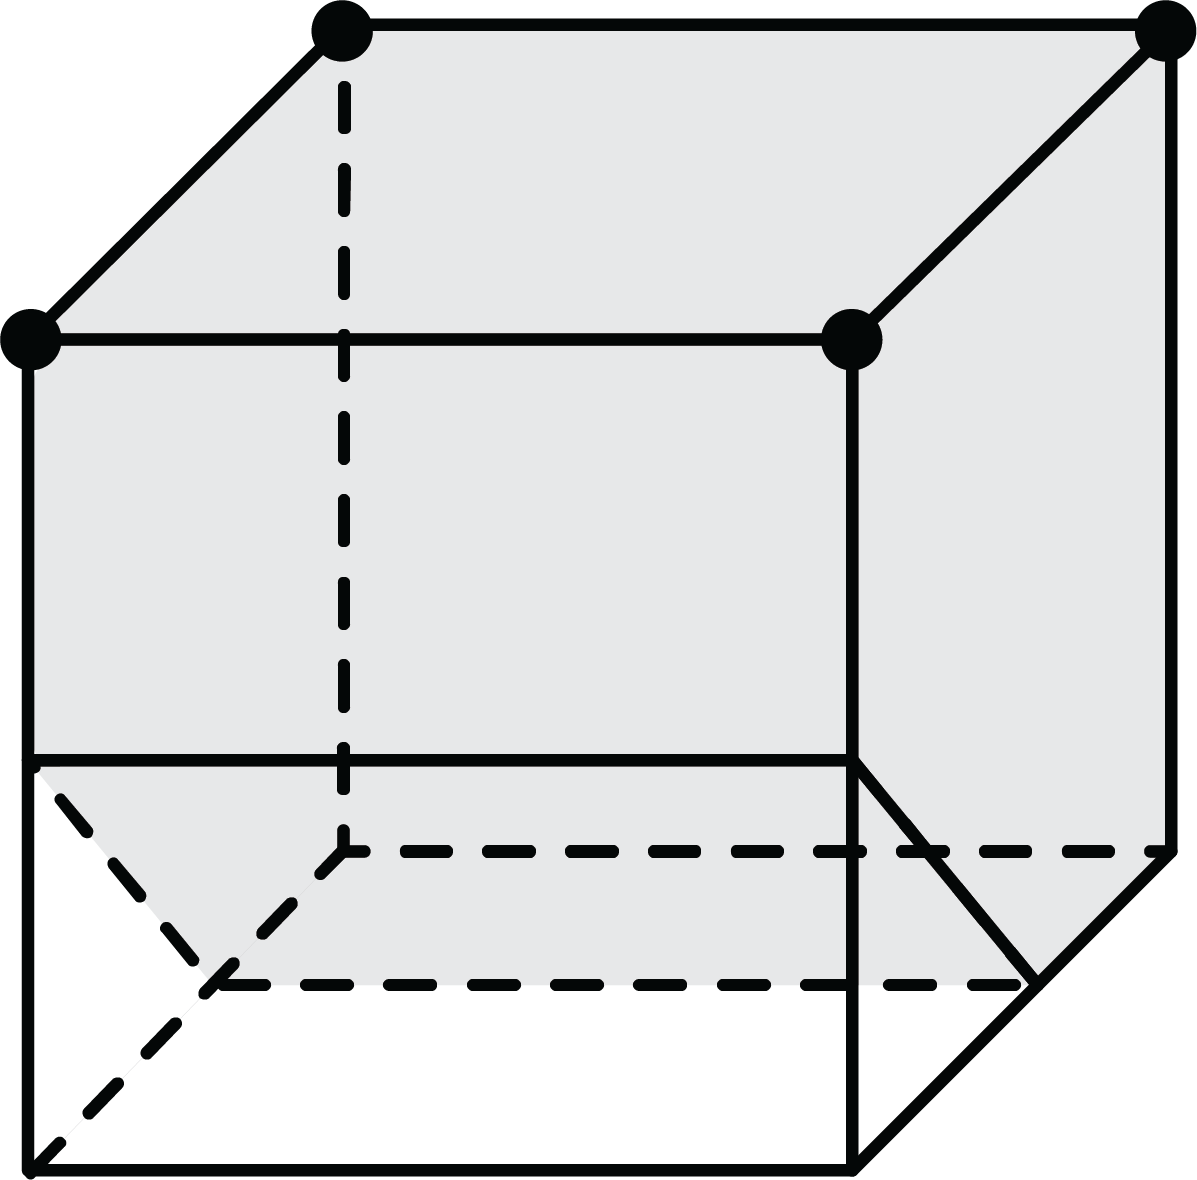
\includegraphics[width=1cm]{Figures/case 18.png} & $\frac{1}{8}$\\

        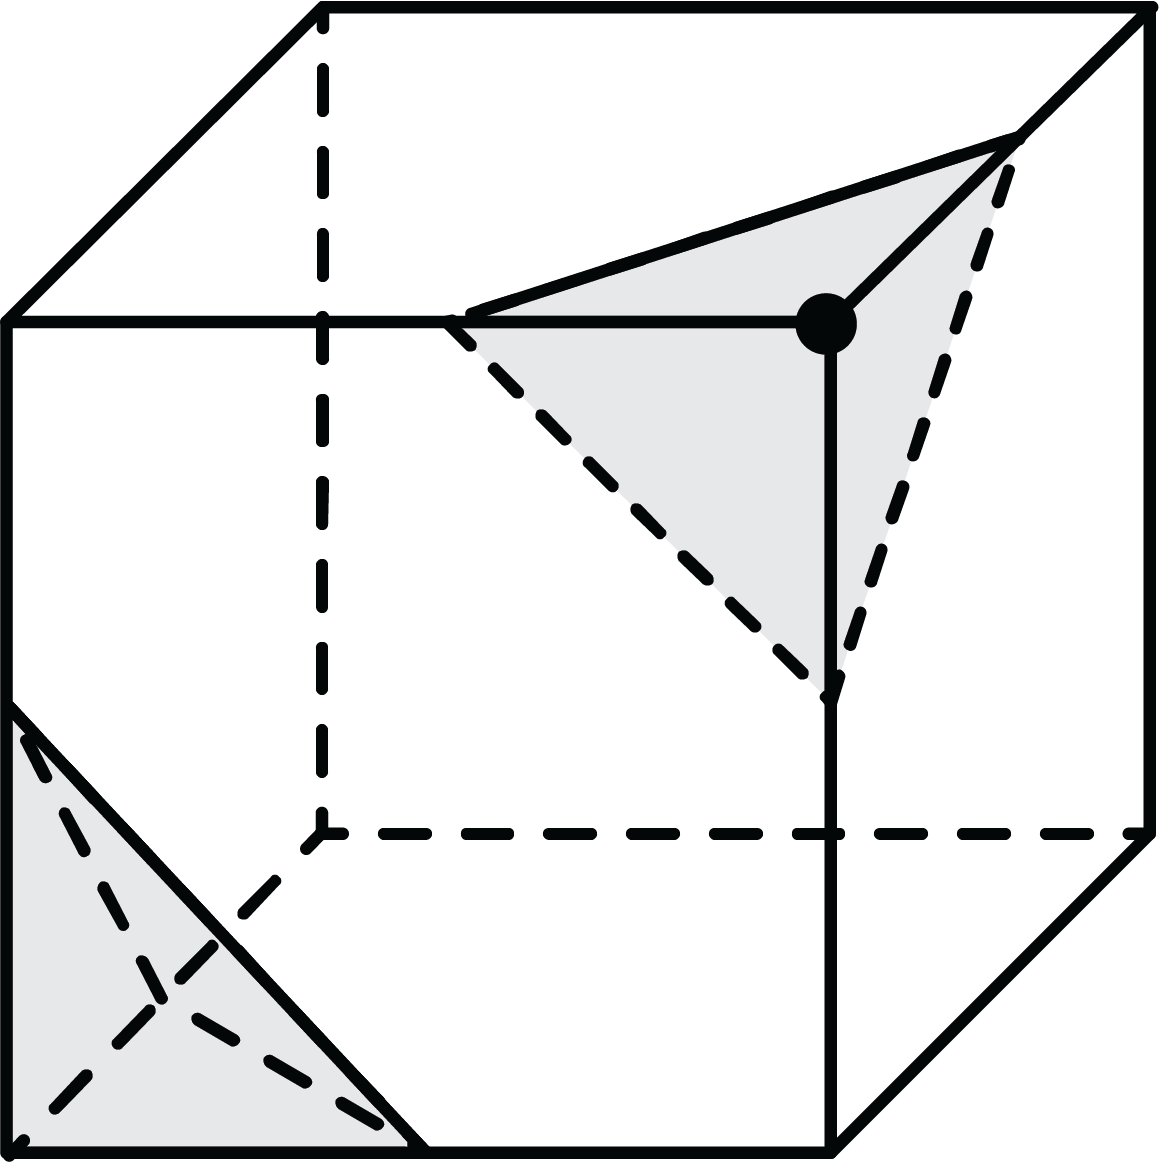
\includegraphics[width=1cm]{Figures/case 4.png} & $2 \times \frac{1}{48}$ & 2 tetrahedrons & $\frac{1}{24}$ & 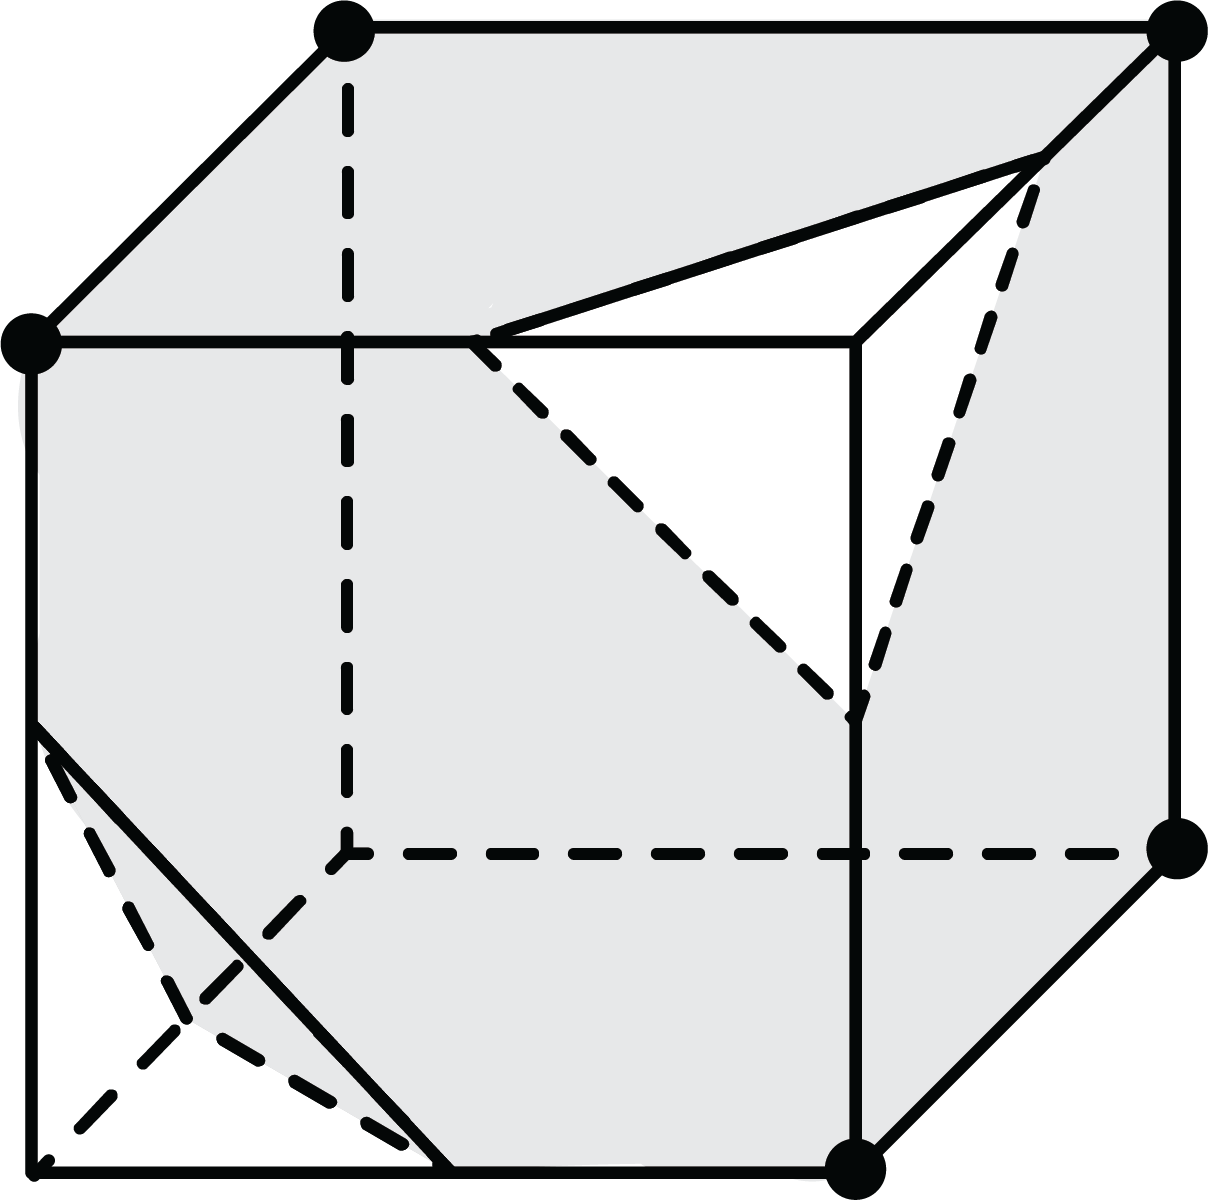
\includegraphics[width=1cm]{Figures/case 19.png} & $\frac{23}{24}$ \\

        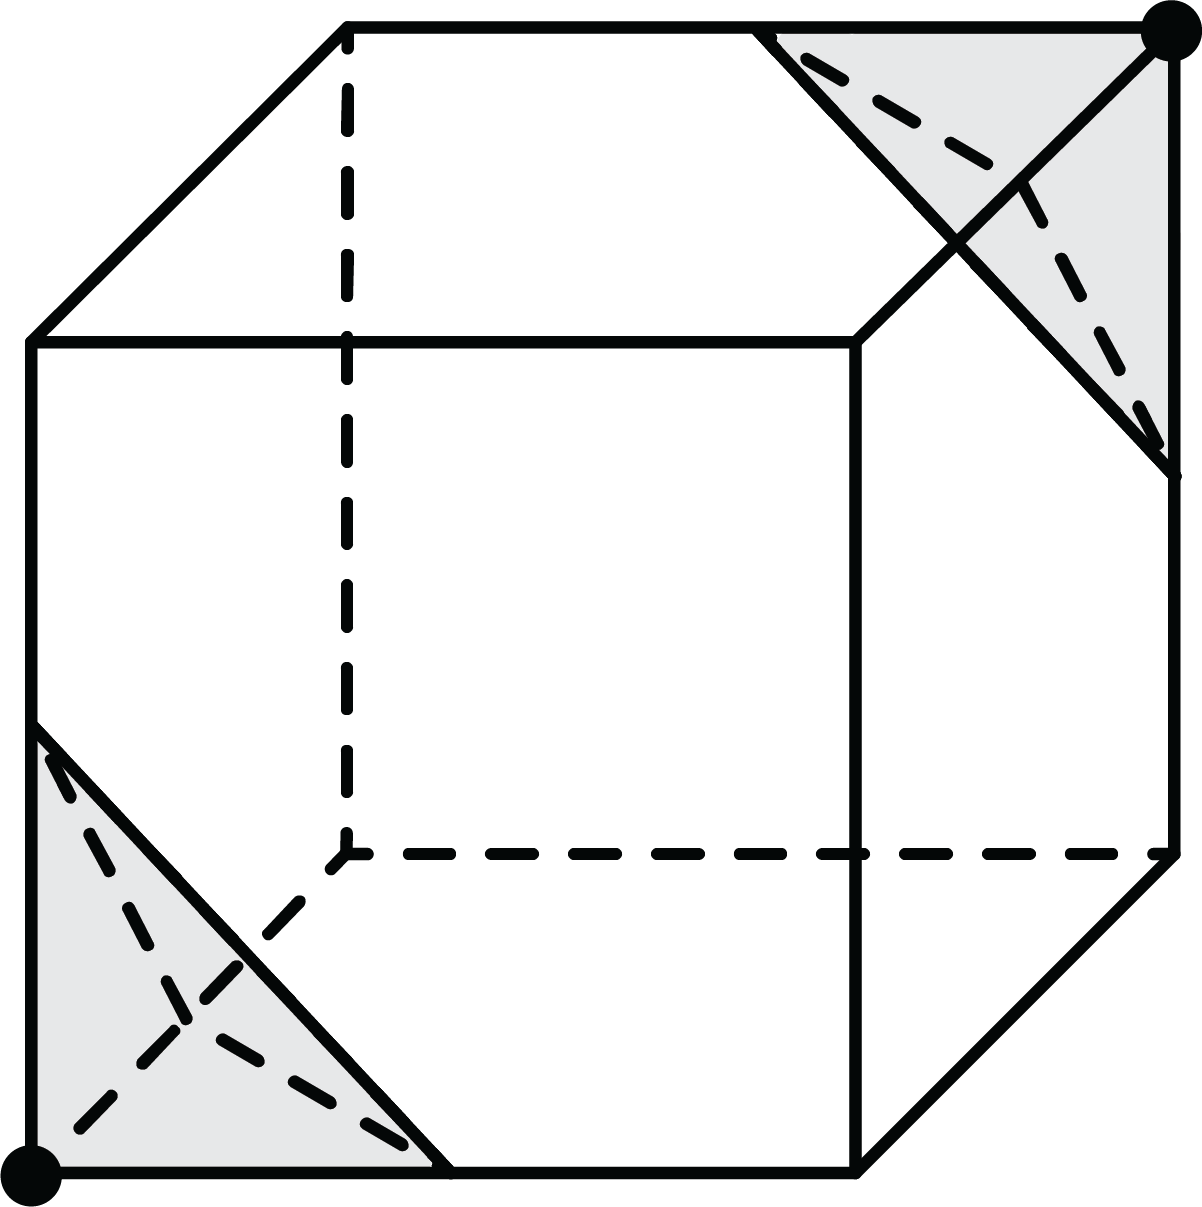
\includegraphics[width=1cm]{Figures/case 5.png} & $2 \times \frac{1}{48}$ & 2 tetrahedrons & $\frac{1}{24}$ & 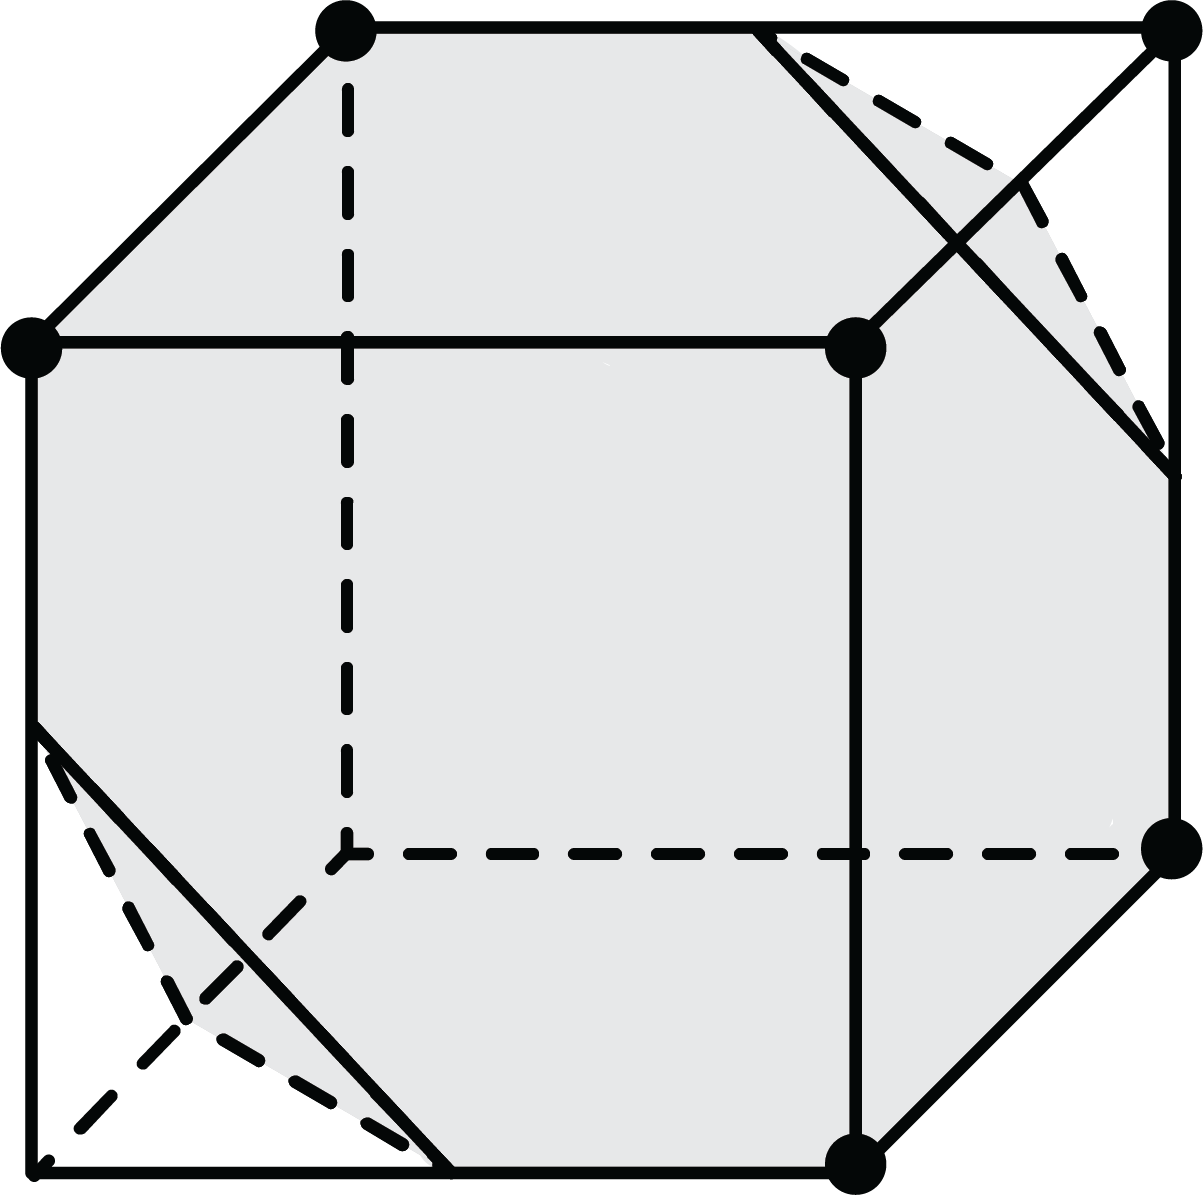
\includegraphics[width=1cm]{Figures/case 20.png} & $\frac{23}{24}$ \\

        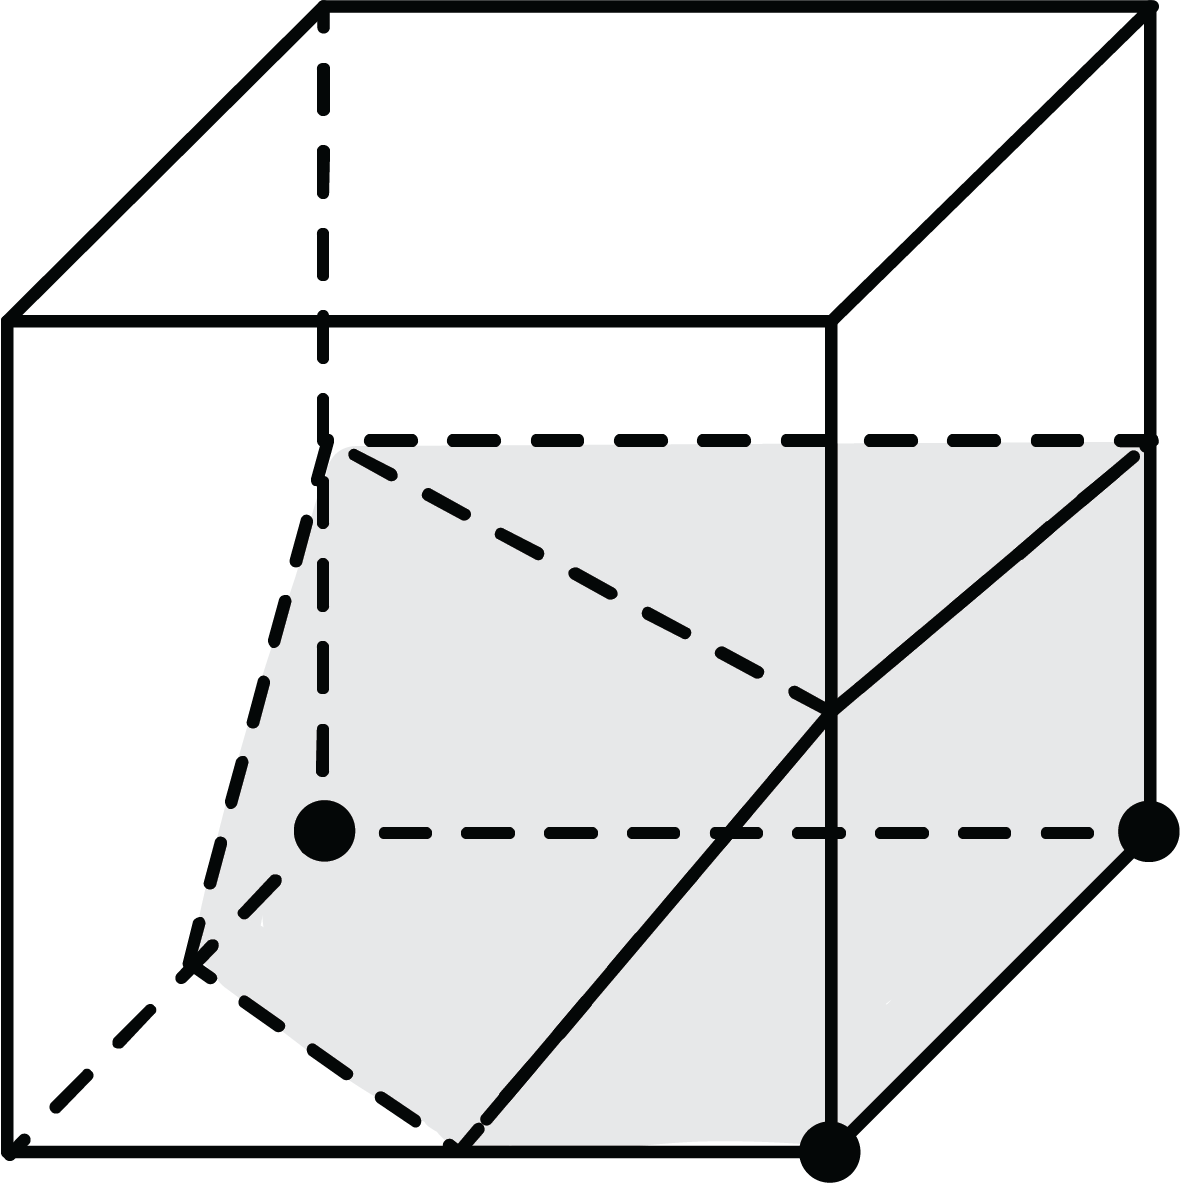
\includegraphics[width=1cm]{Figures/case 6.png} & $\frac{1}{4} + \frac{1}{12} + \frac{1}{48}$ & 1 prism, 2 tetrahedrons & $\frac{17}{48}$ & 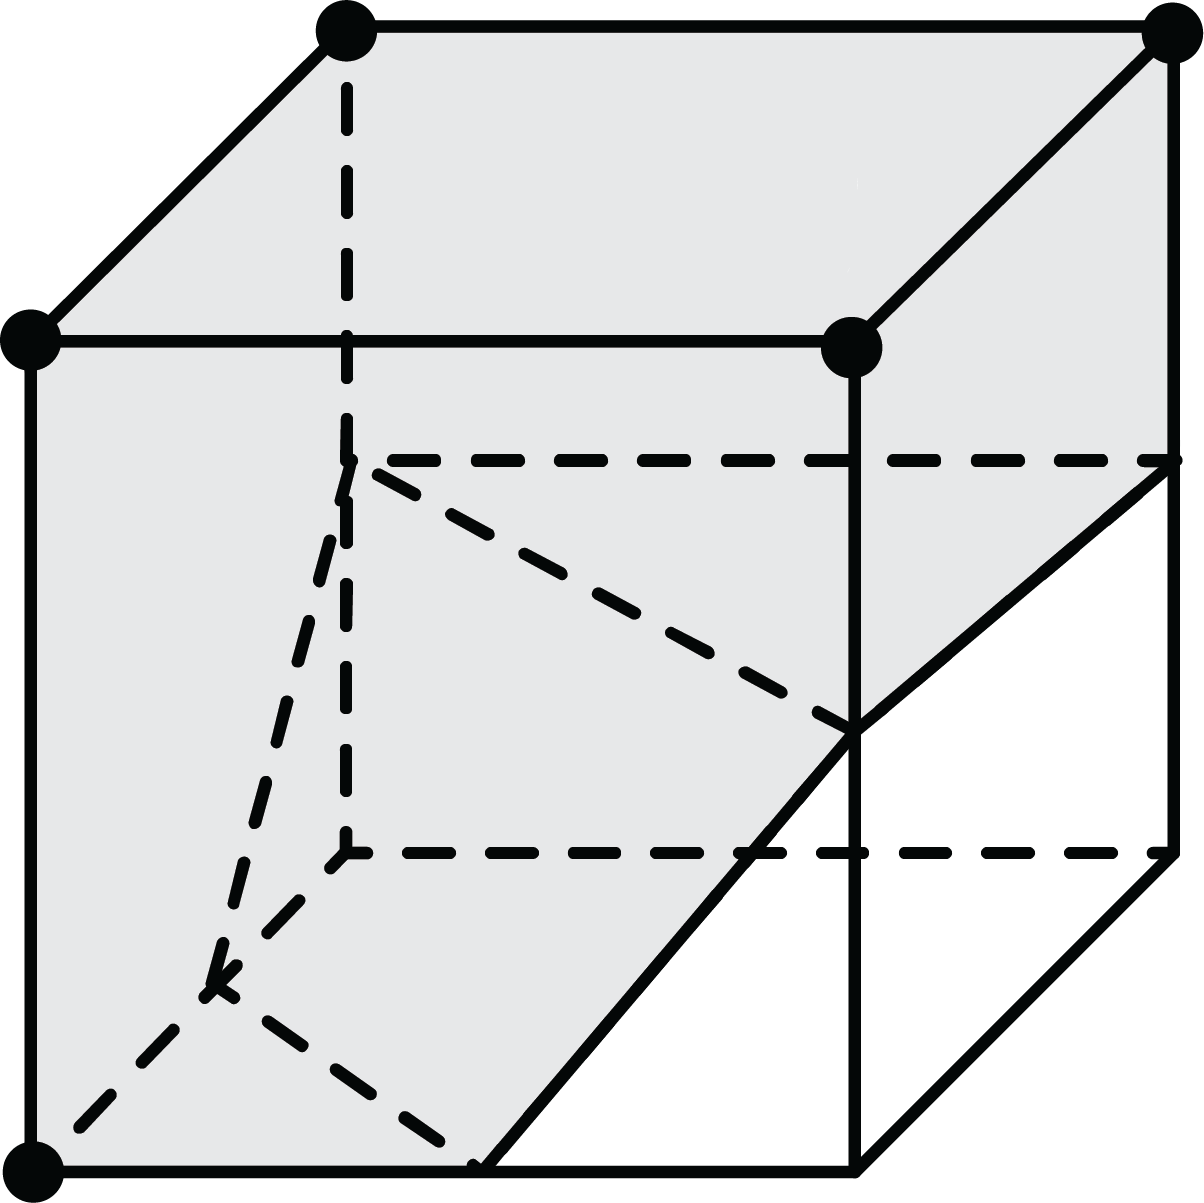
\includegraphics[width=1cm]{Figures/case 21.png} & $\frac{31}{48}$ \\

        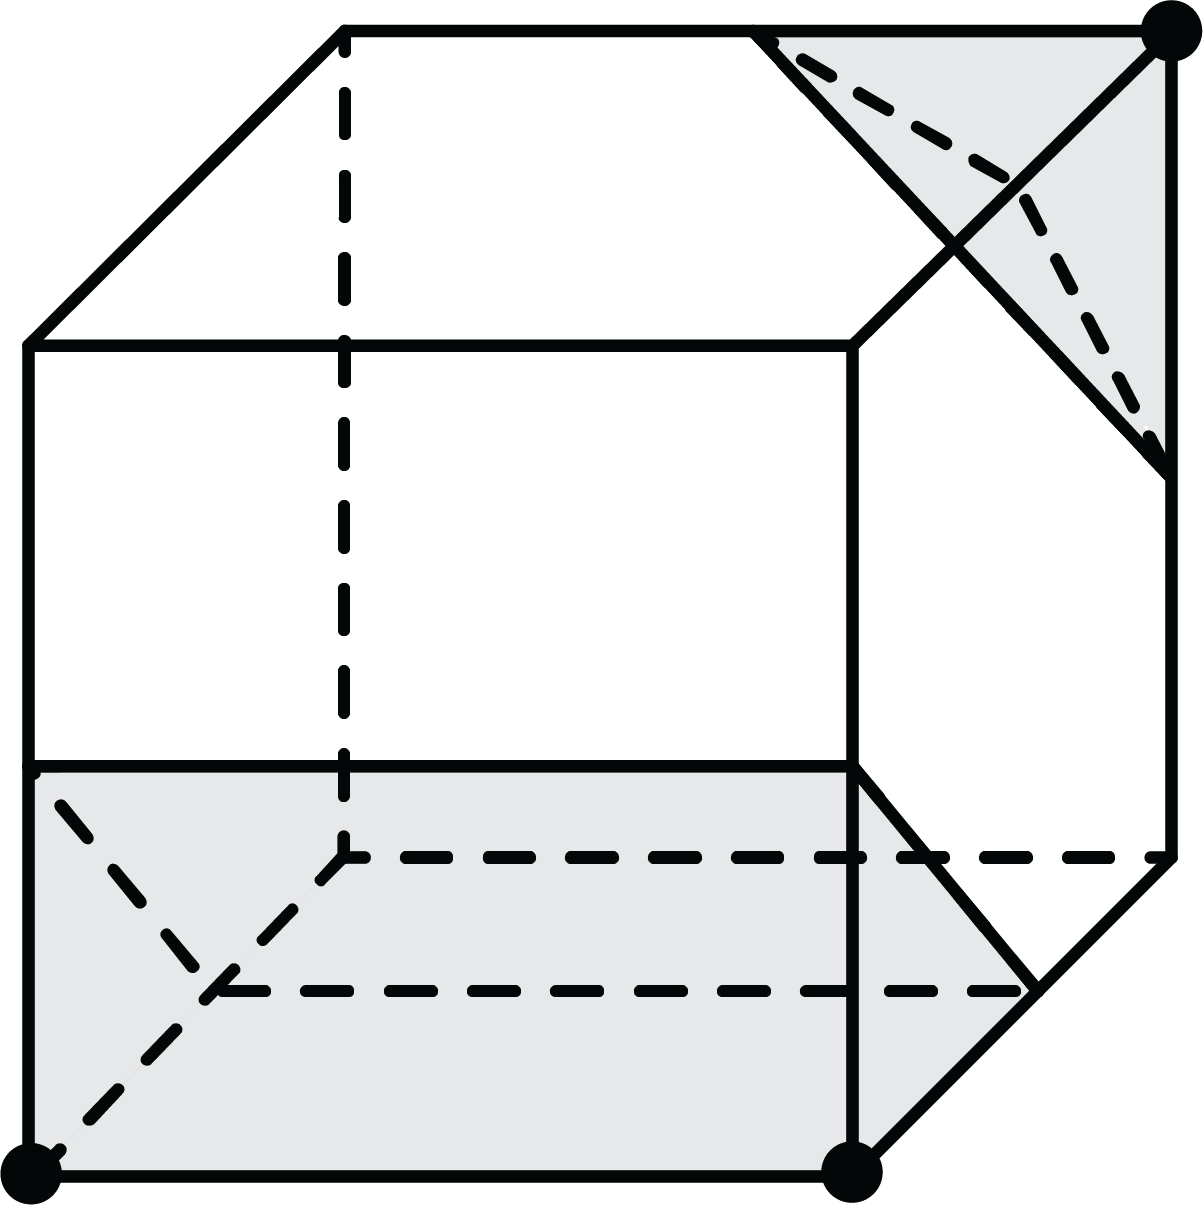
\includegraphics[width=1cm]{Figures/case 7.png} & $\frac{1}{8} + \frac{1}{48}$ & 1 prism, 1 tetrahedron & $\frac{7}{48}$ & 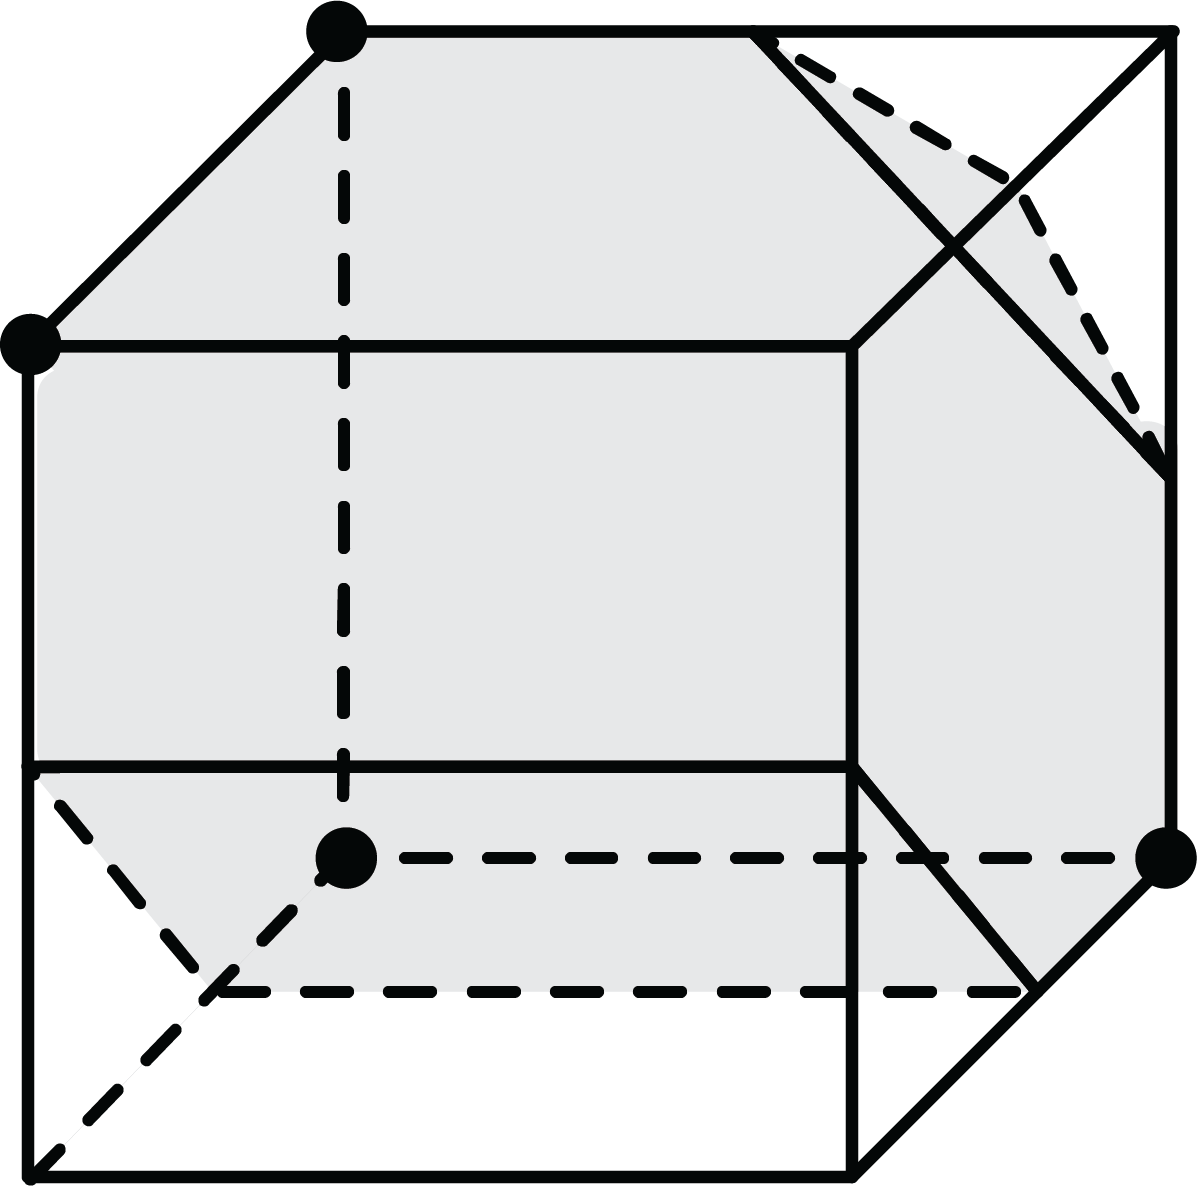
\includegraphics[width=1cm]{Figures/case 22.png} & $\frac{41}{48}$ \\

        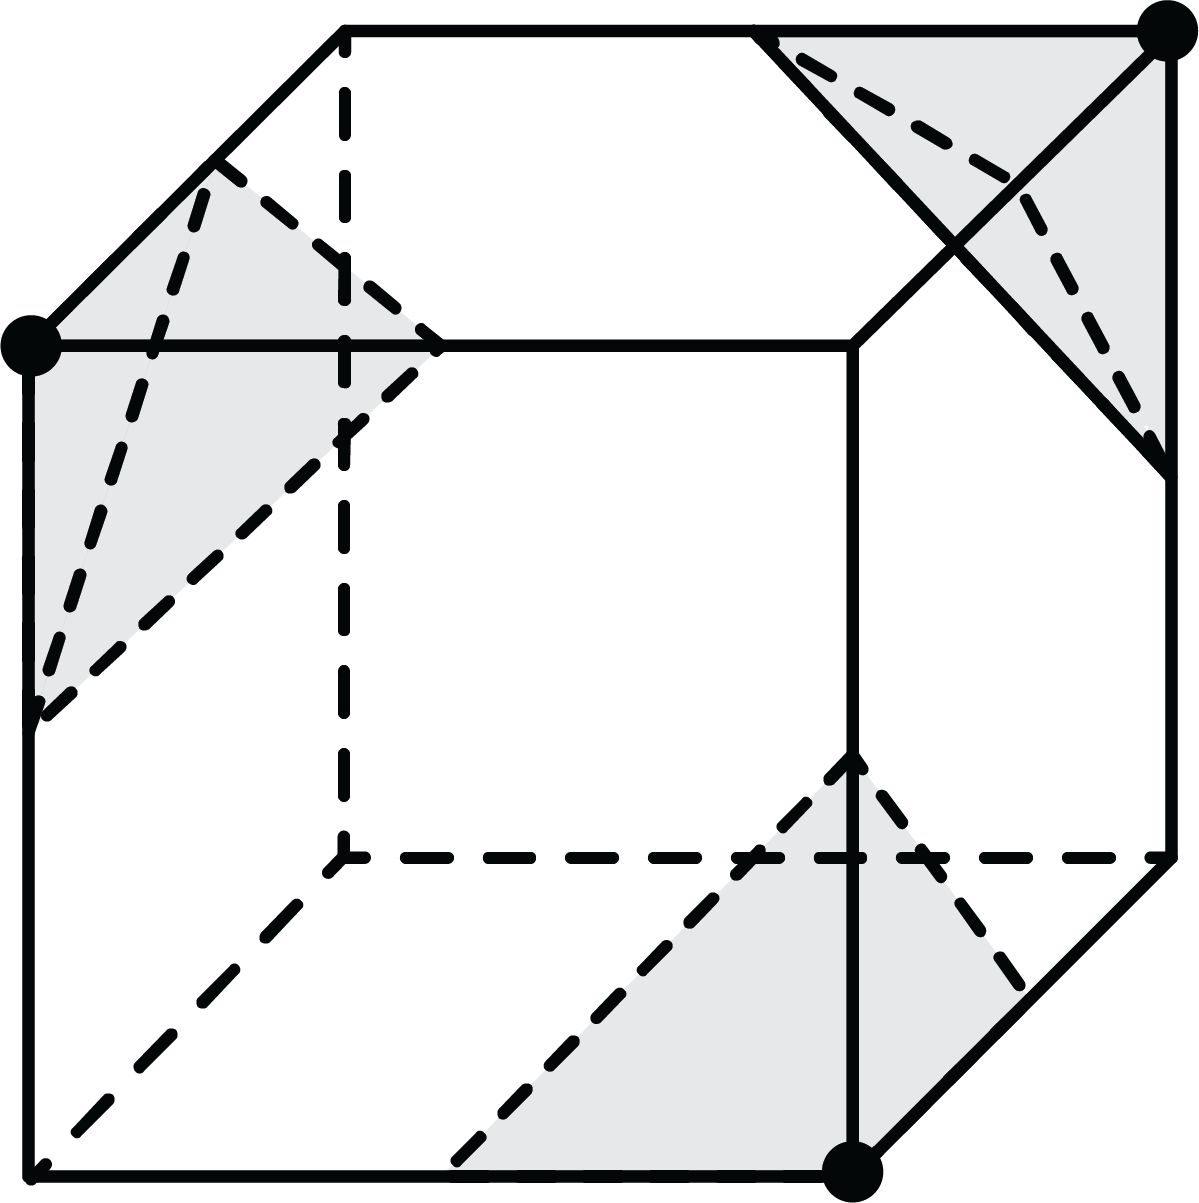
\includegraphics[width=1cm]{Figures/case 8.png} & $3 \times \frac{1}{48}$ & 3 tetrahedrons & $\frac{1}{16}$ & 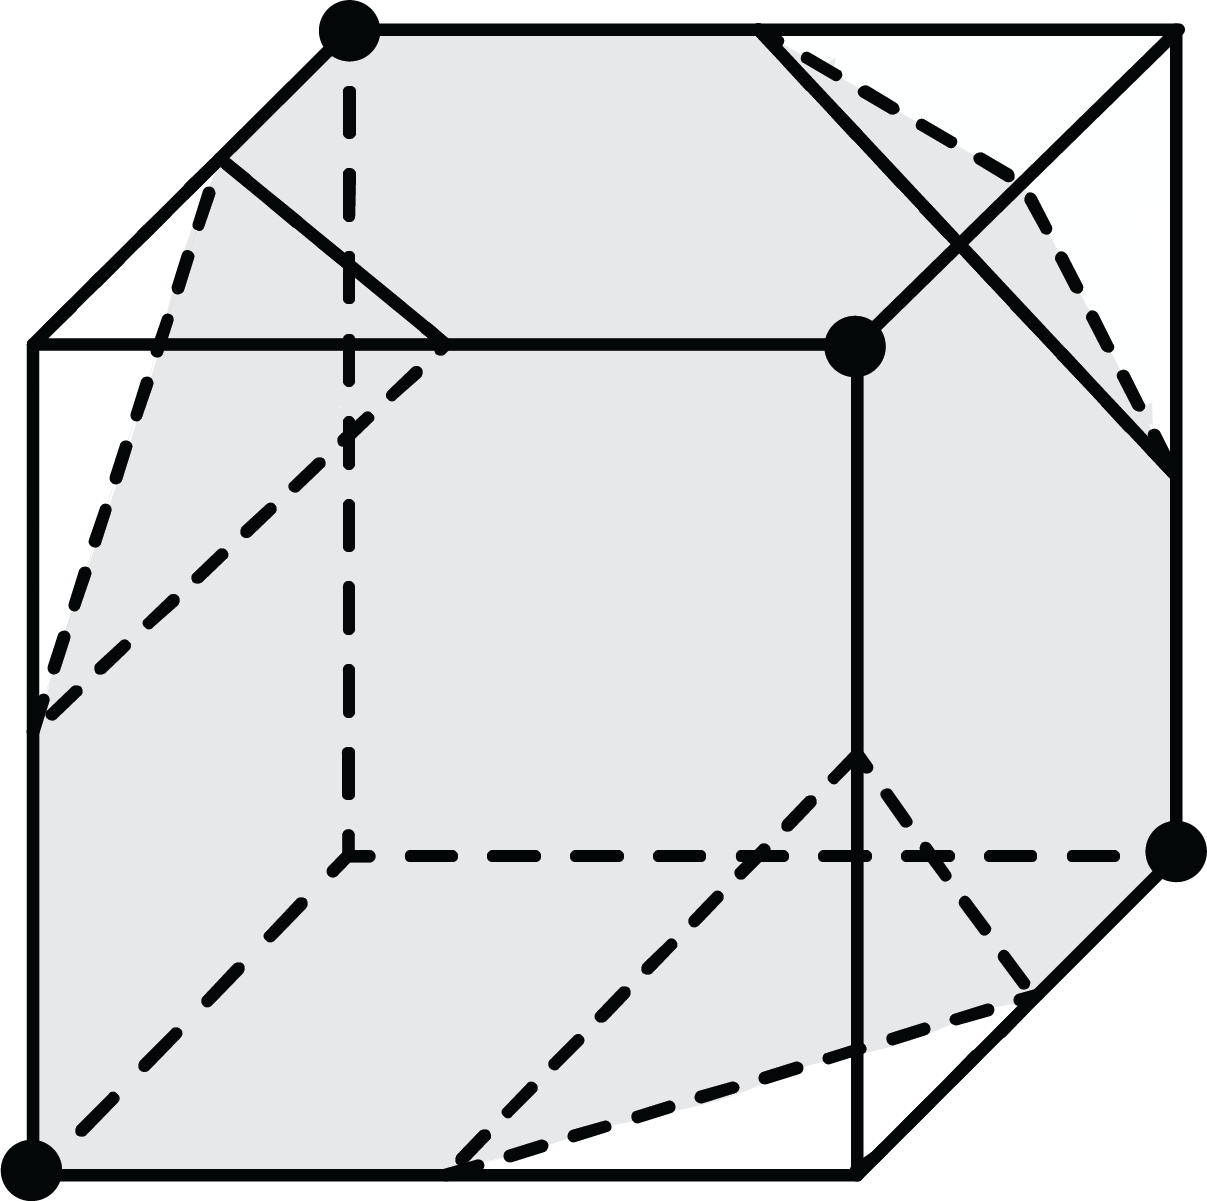
\includegraphics[width=1cm]{Figures/case 23.png} & $\frac{15}{16}$ \\

        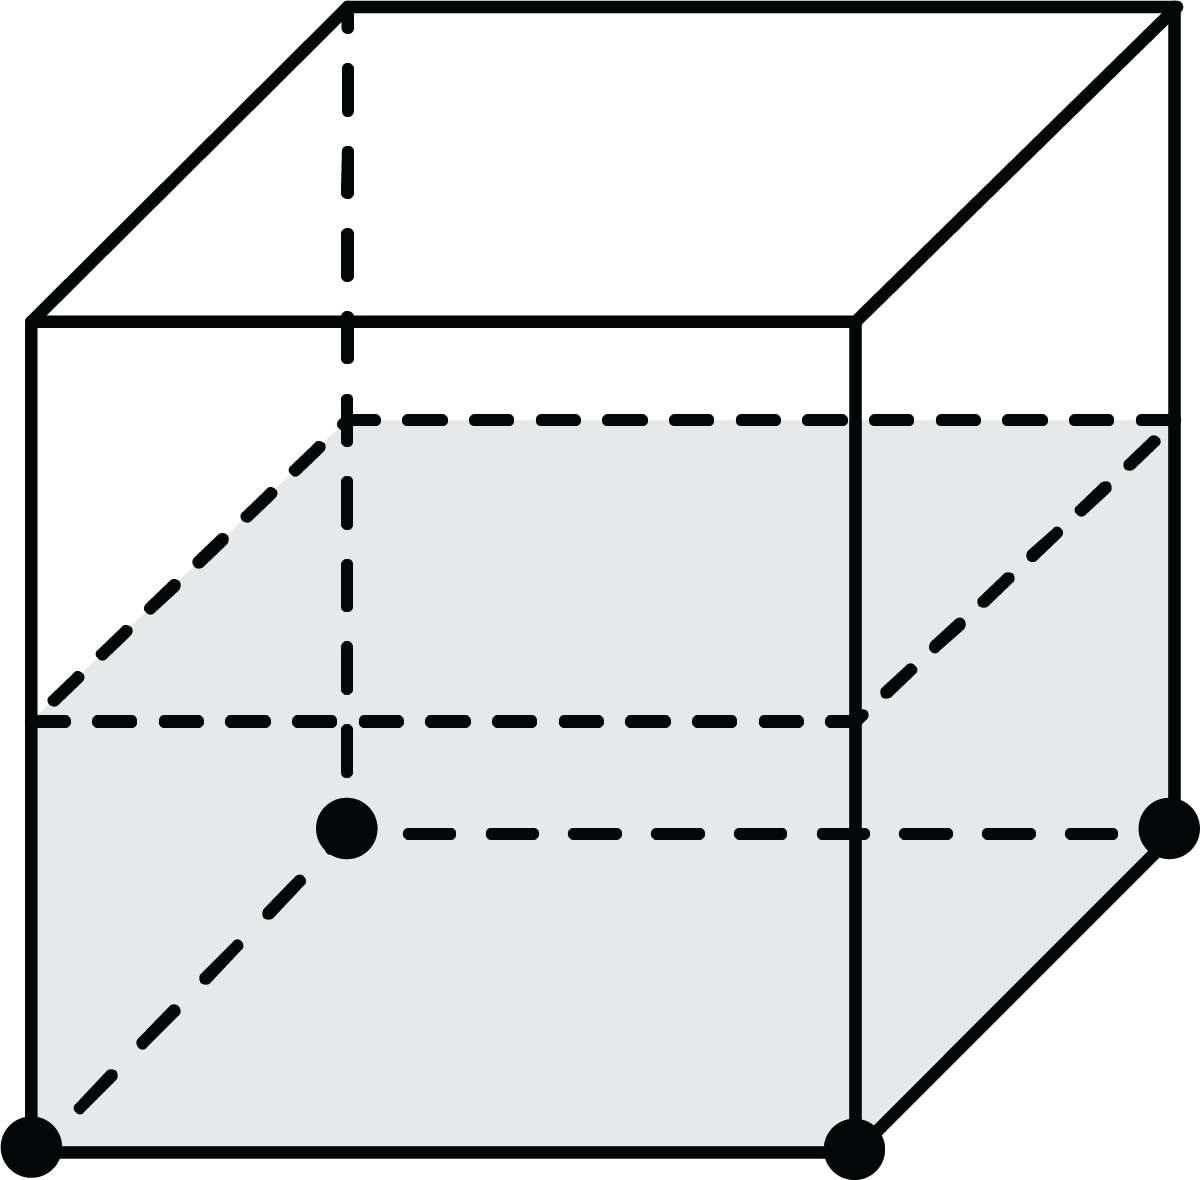
\includegraphics[width=1cm]{Figures/case 9.png} & $\frac{1}{2}$ & half of 1 cube & $\frac{1}{2}$ & 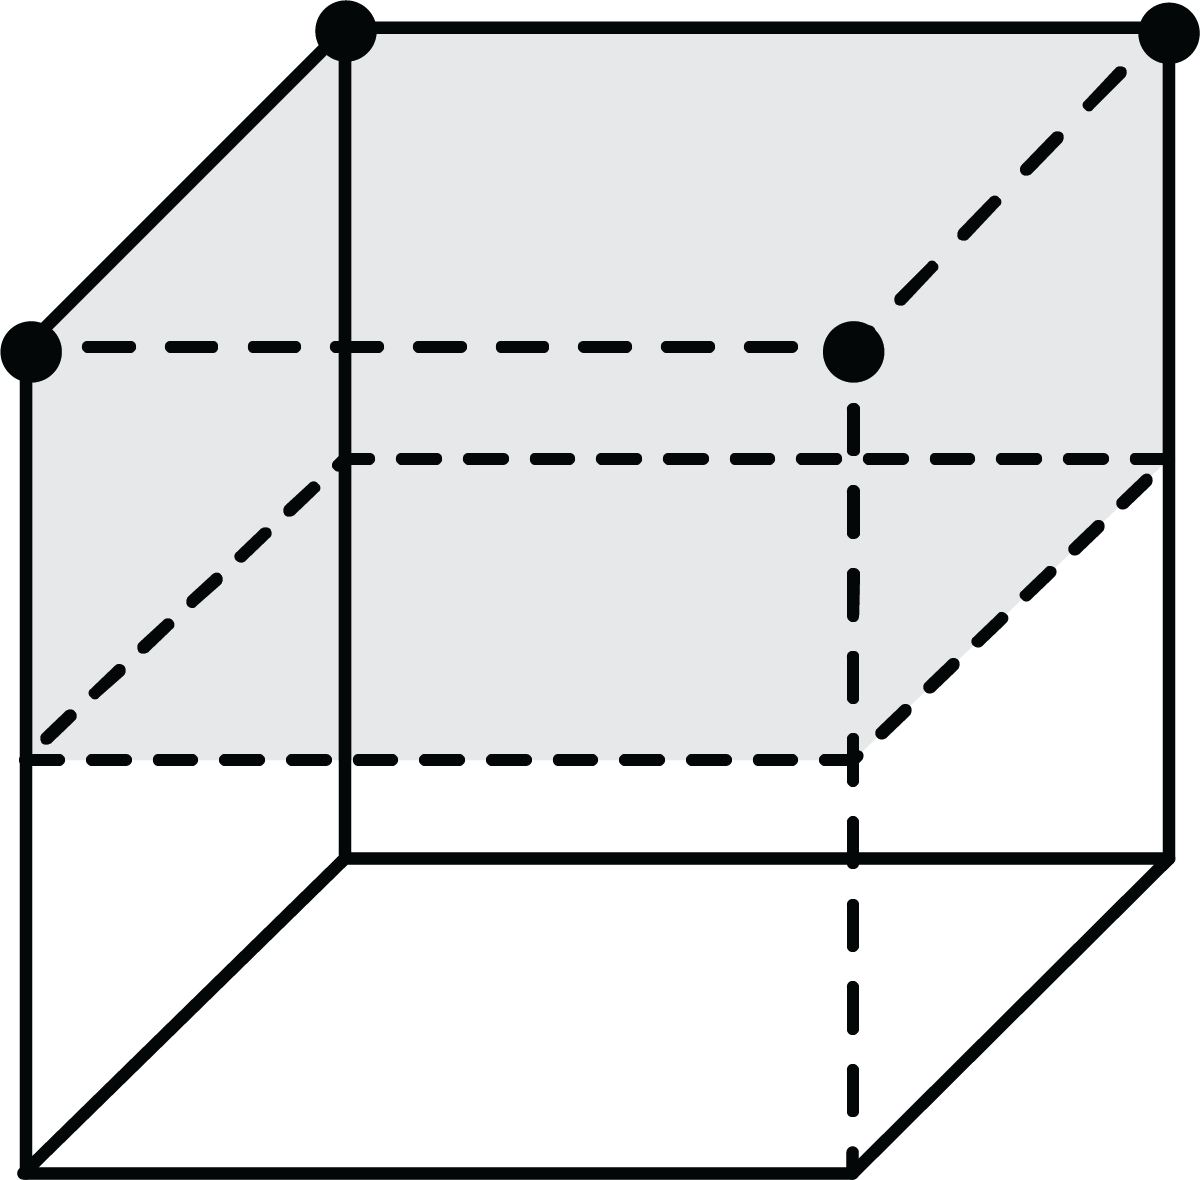
\includegraphics[width=1cm]{Figures/case 24.png} & $\frac{1}{2}$ \\

        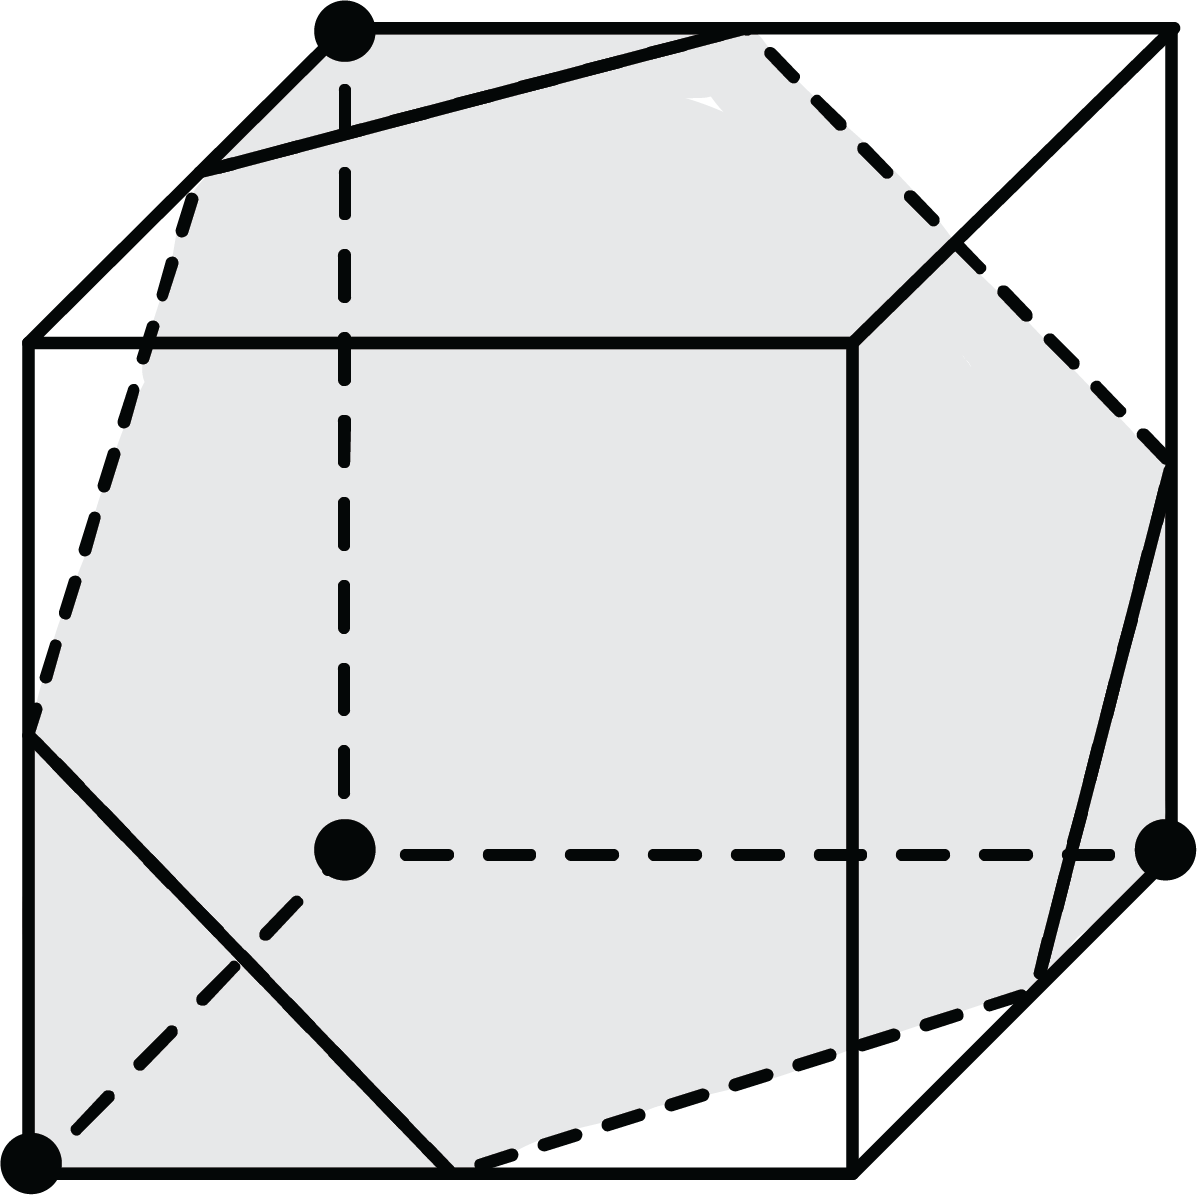
\includegraphics[width=1cm]{Figures/case 10.png} & $\frac{1}{2}$ & half of 1 cube & $\frac{1}{2}$ & 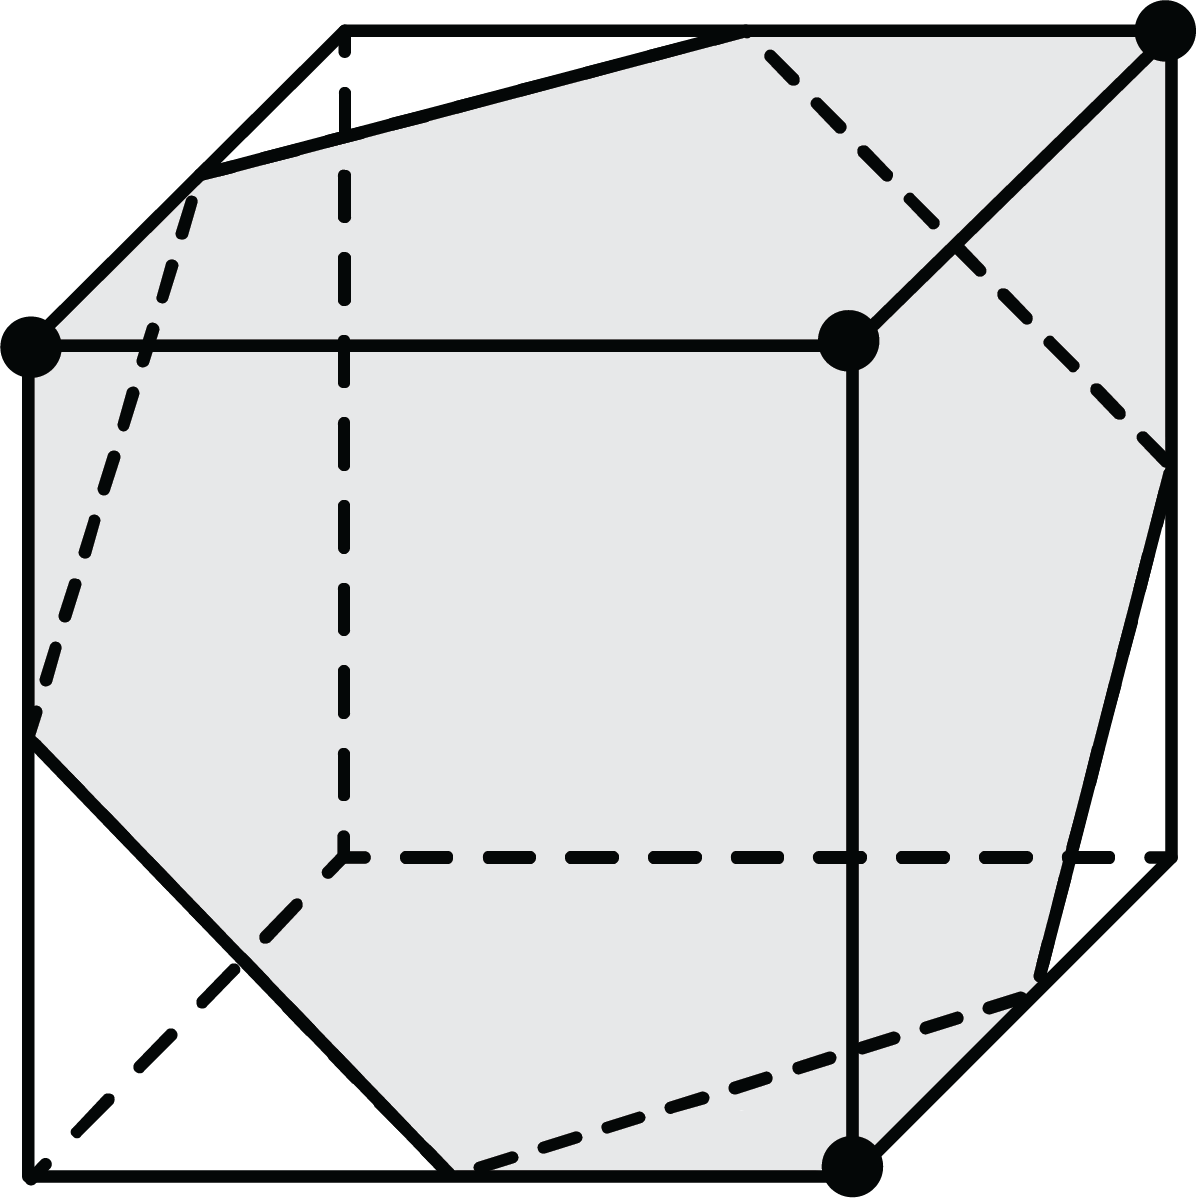
\includegraphics[width=1cm]{Figures/case 25.png} & $\frac{1}{2}$ \\

        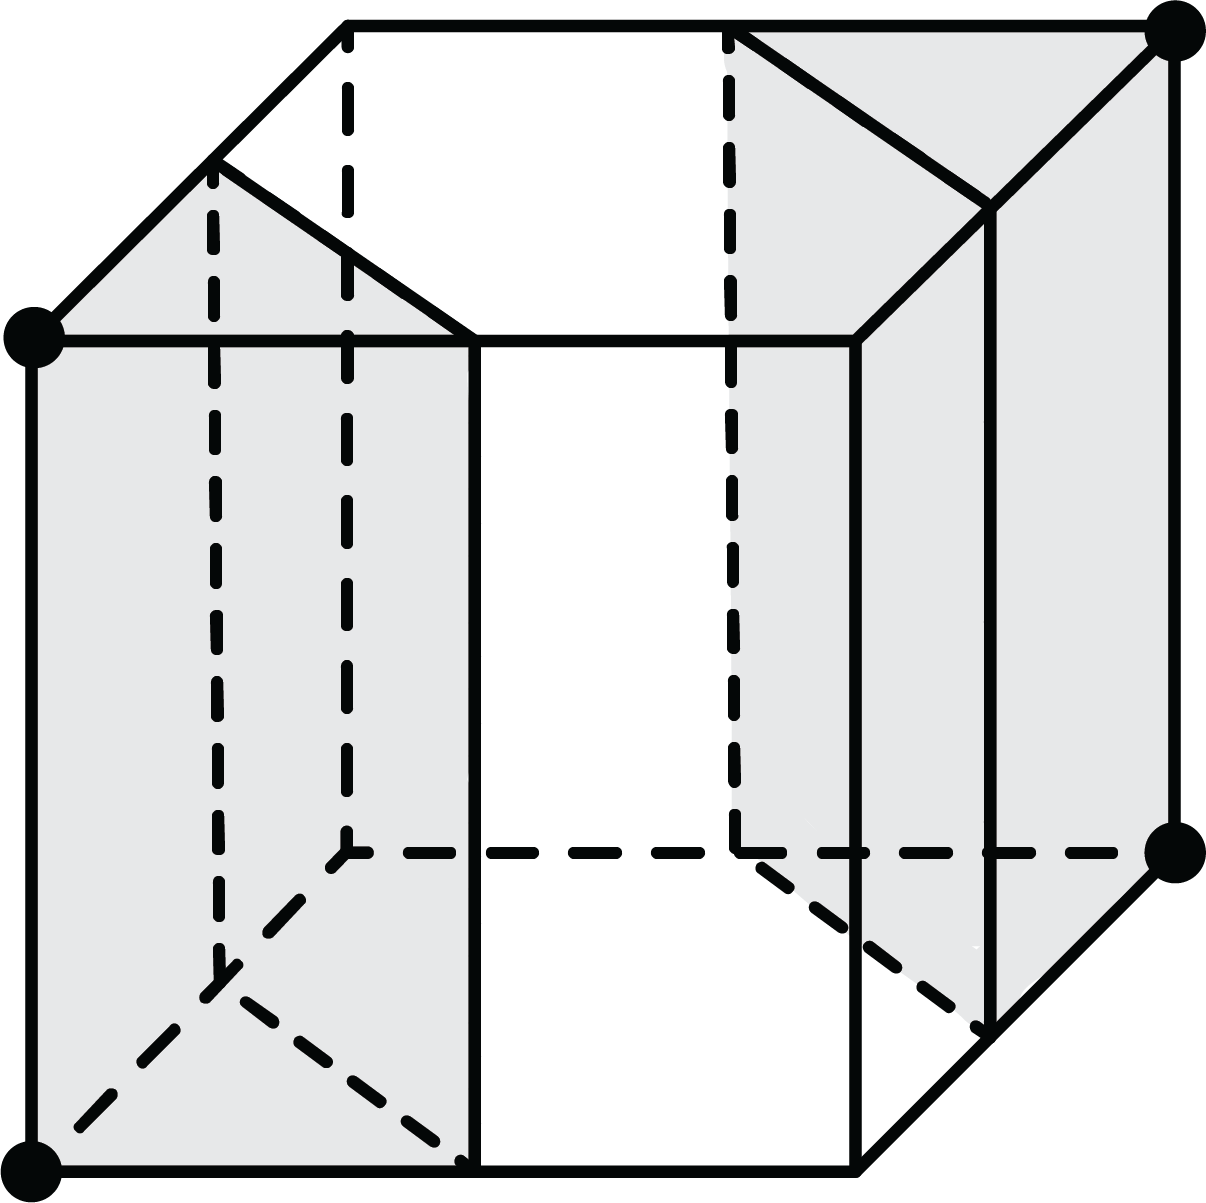
\includegraphics[width=1cm]{Figures/case 11.png} & $2 \times \frac{1}{8}$ & 2 prisms & $\frac{1}{4}$ & 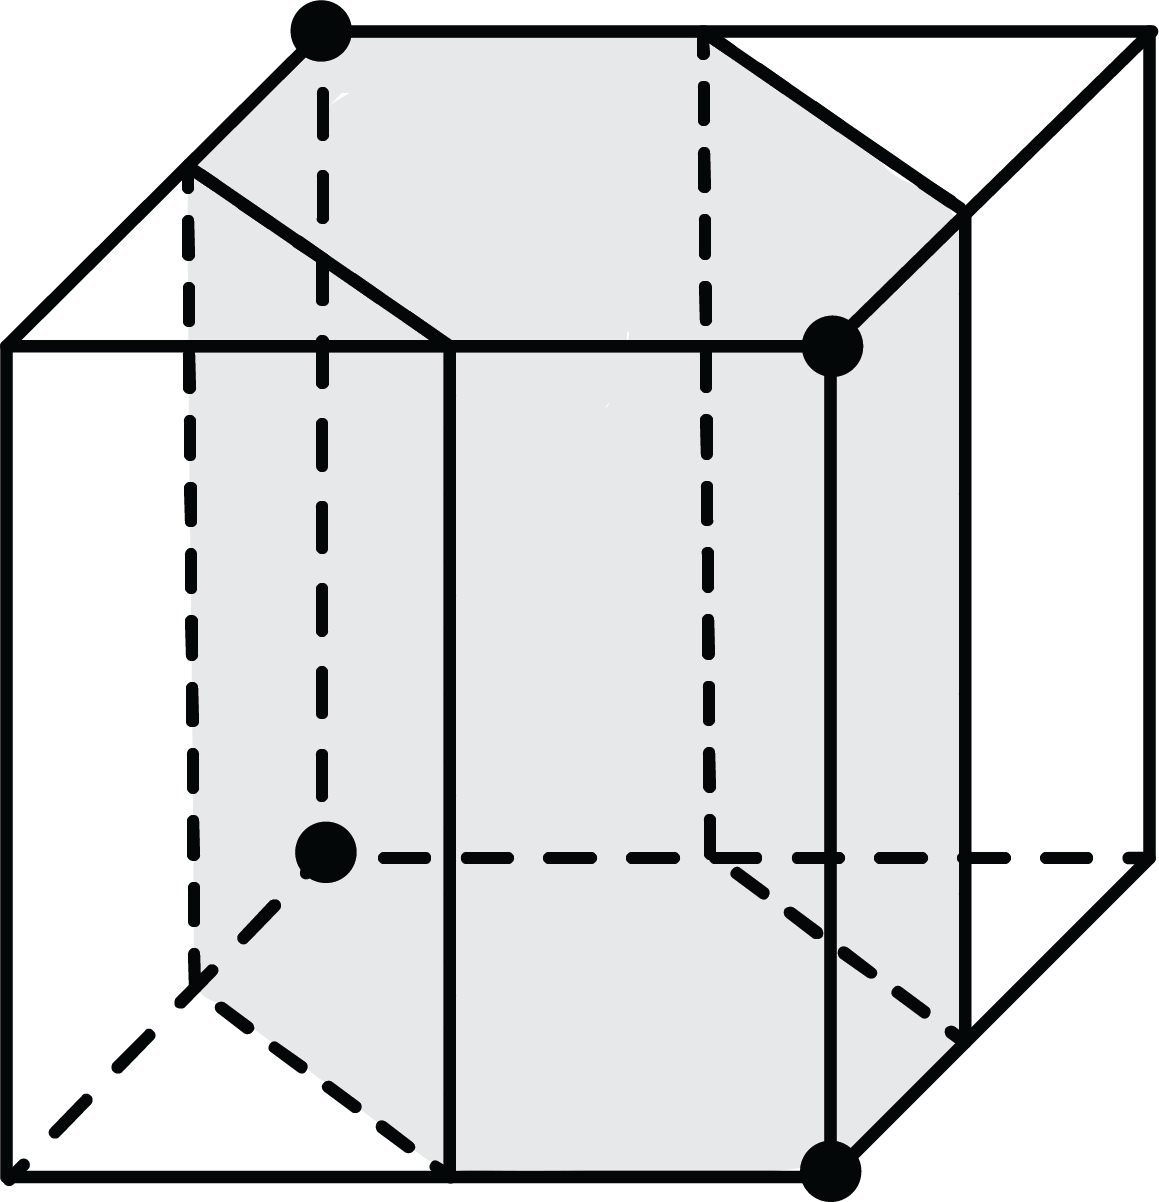
\includegraphics[width=1cm]{Figures/case 26.png} & $\frac{3}{4}$ \\

        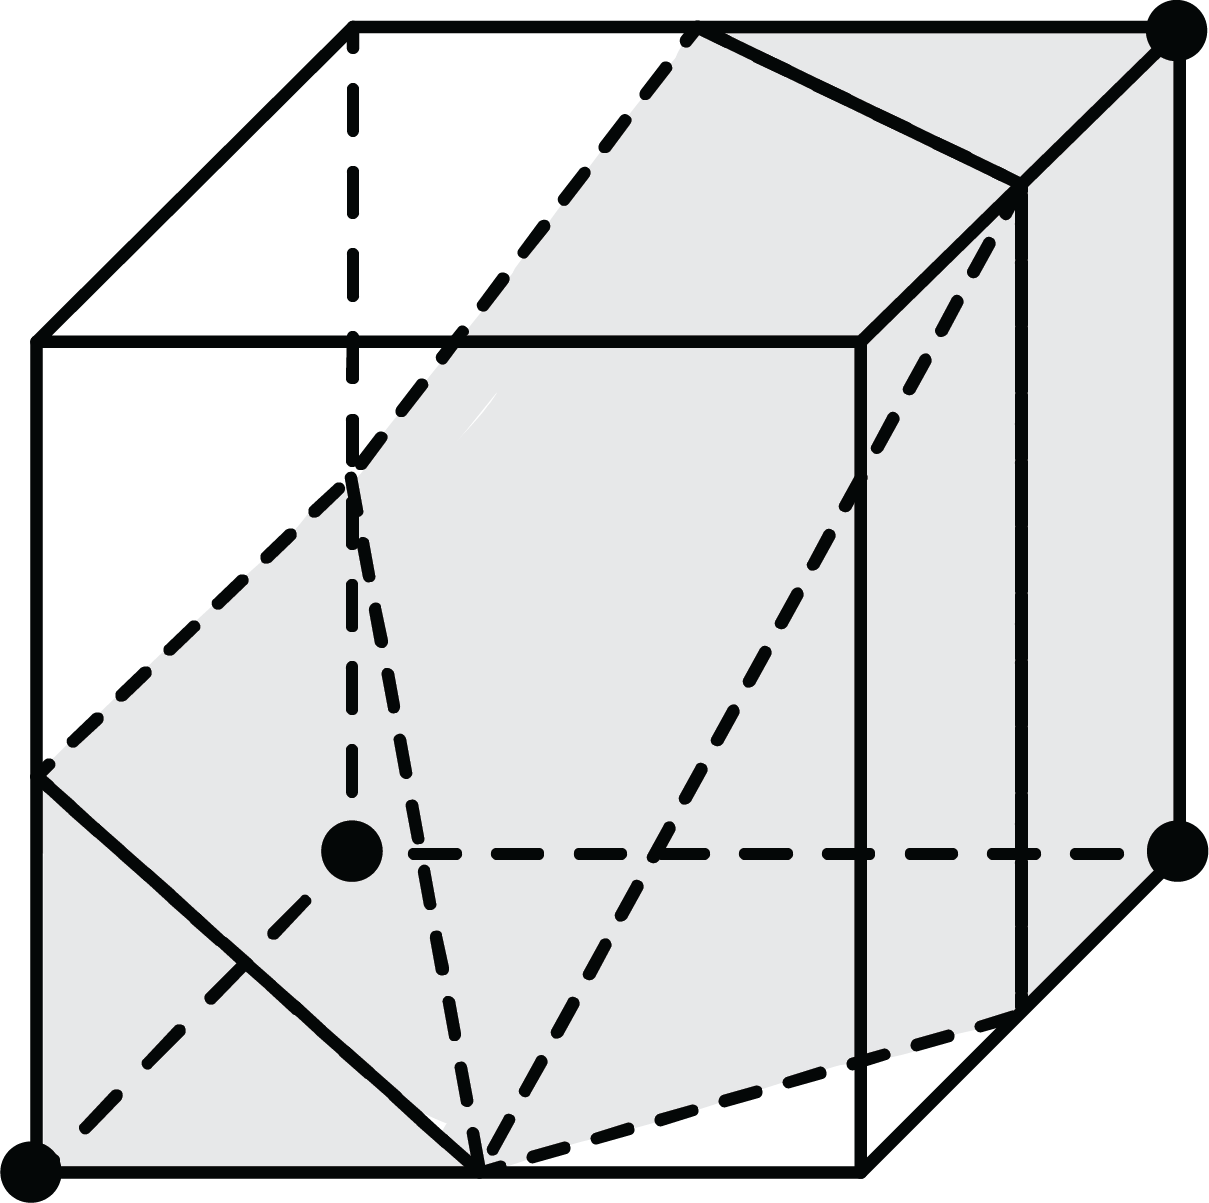
\includegraphics[width=1cm]{Figures/case 12.png} & $\frac{1}{8} + \frac{1}{12} + \frac{1}{6} + \frac{1}{8}$ & 1 prism, 3 tetrahedrons & $\frac{1}{2}$ & 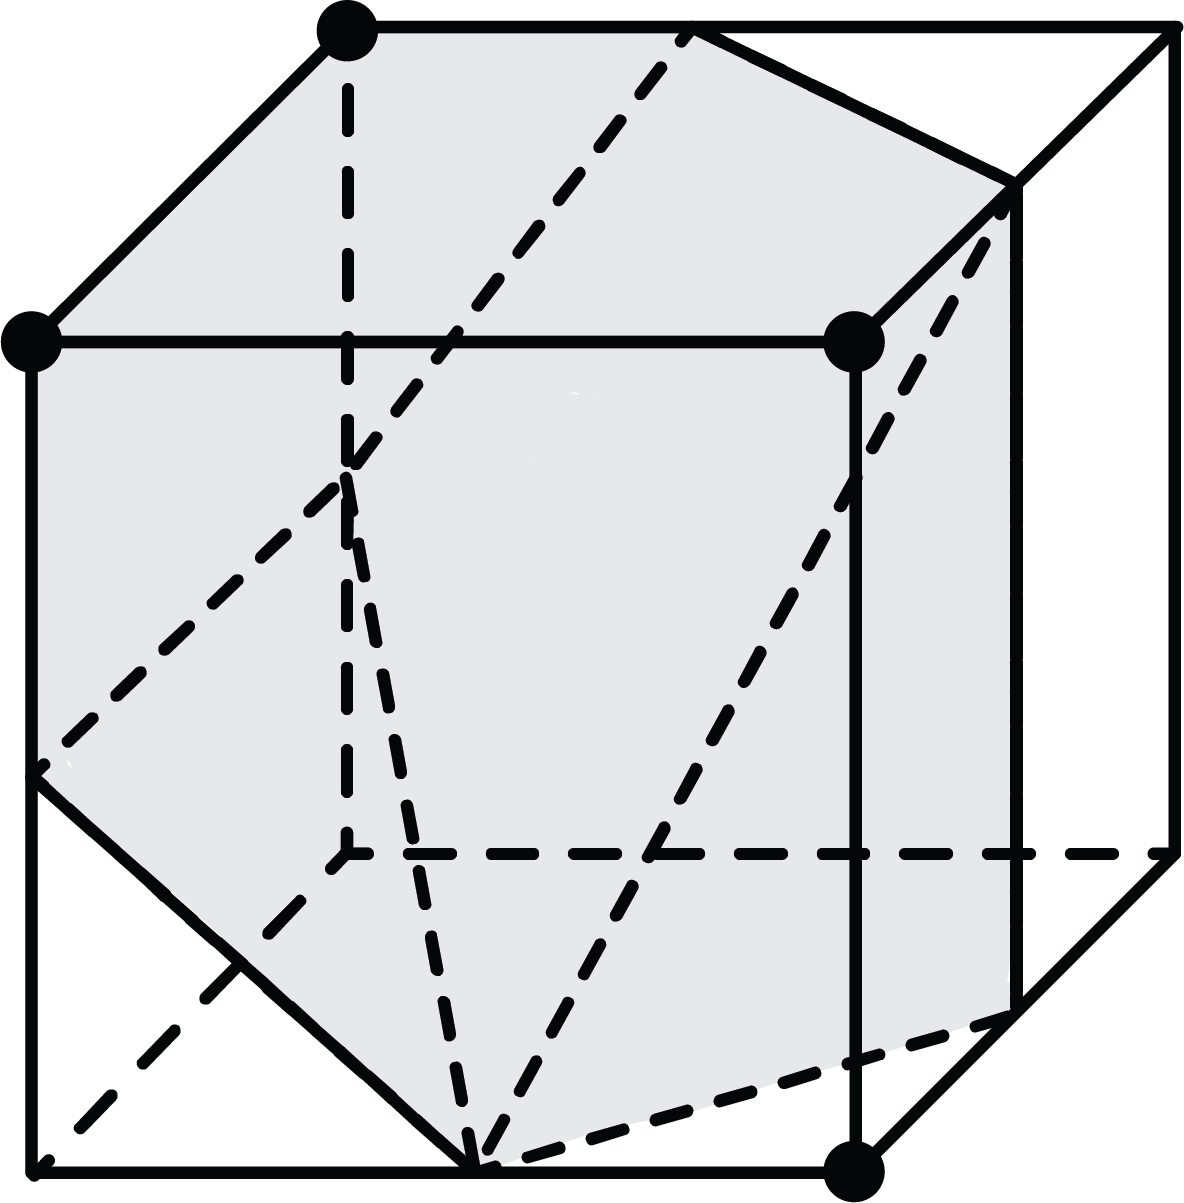
\includegraphics[width=1cm]{Figures/case 27.png} & $\frac{1}{2}$ \\

        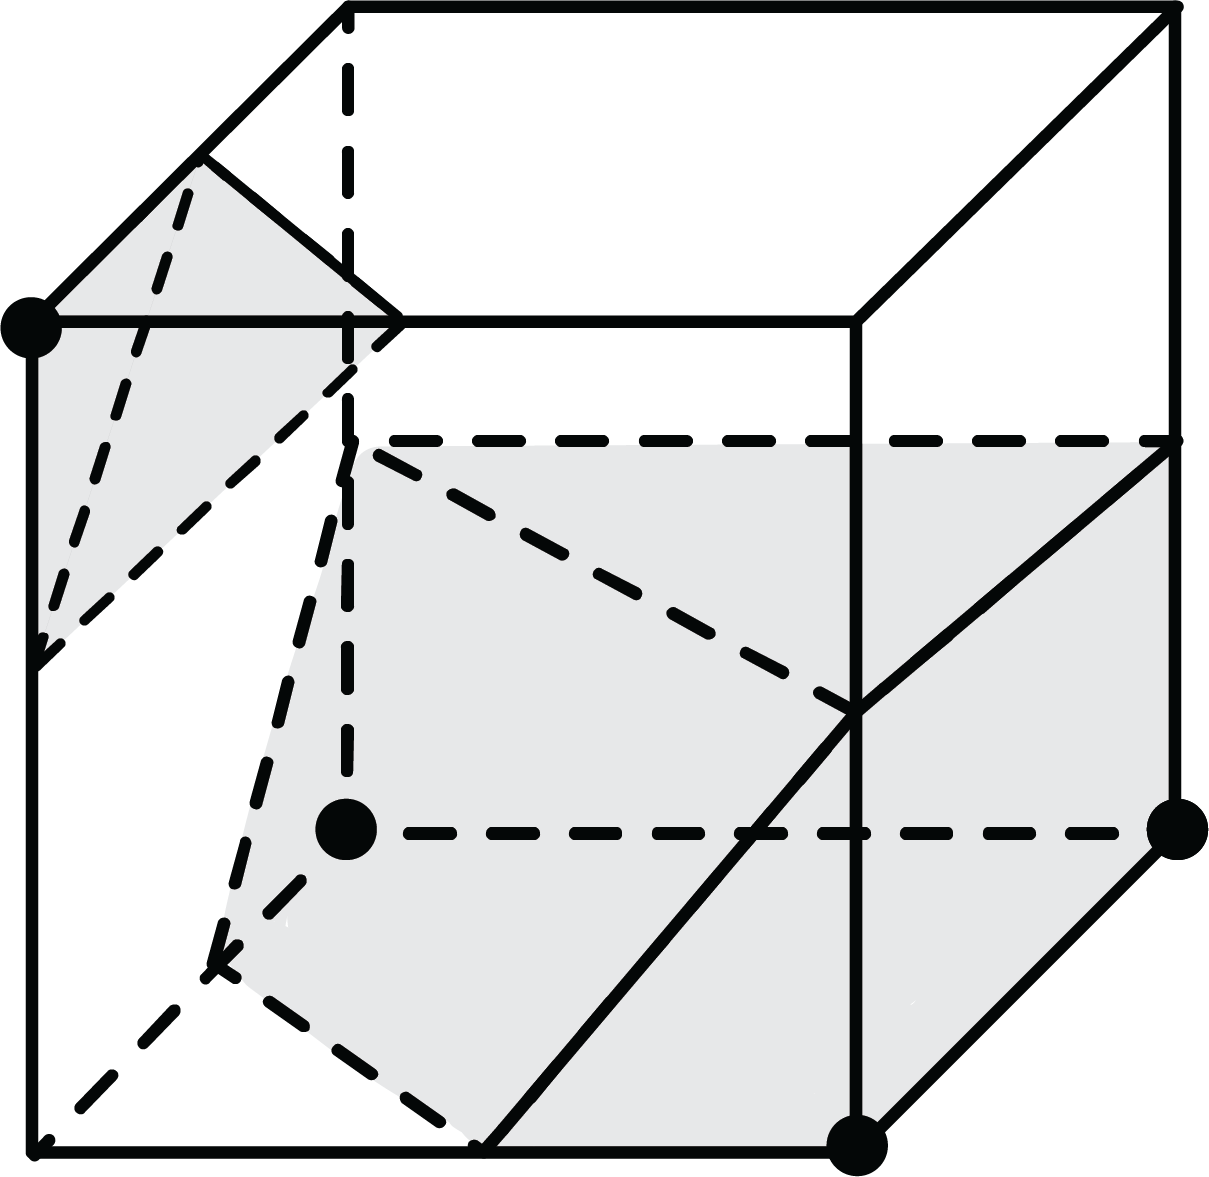
\includegraphics[width=1cm]{Figures/case 13.png} & $\frac{1}{48} + \frac{17}{48}$ &1 prism, 3 tetrahedrons& $\frac{139}{144}$ & 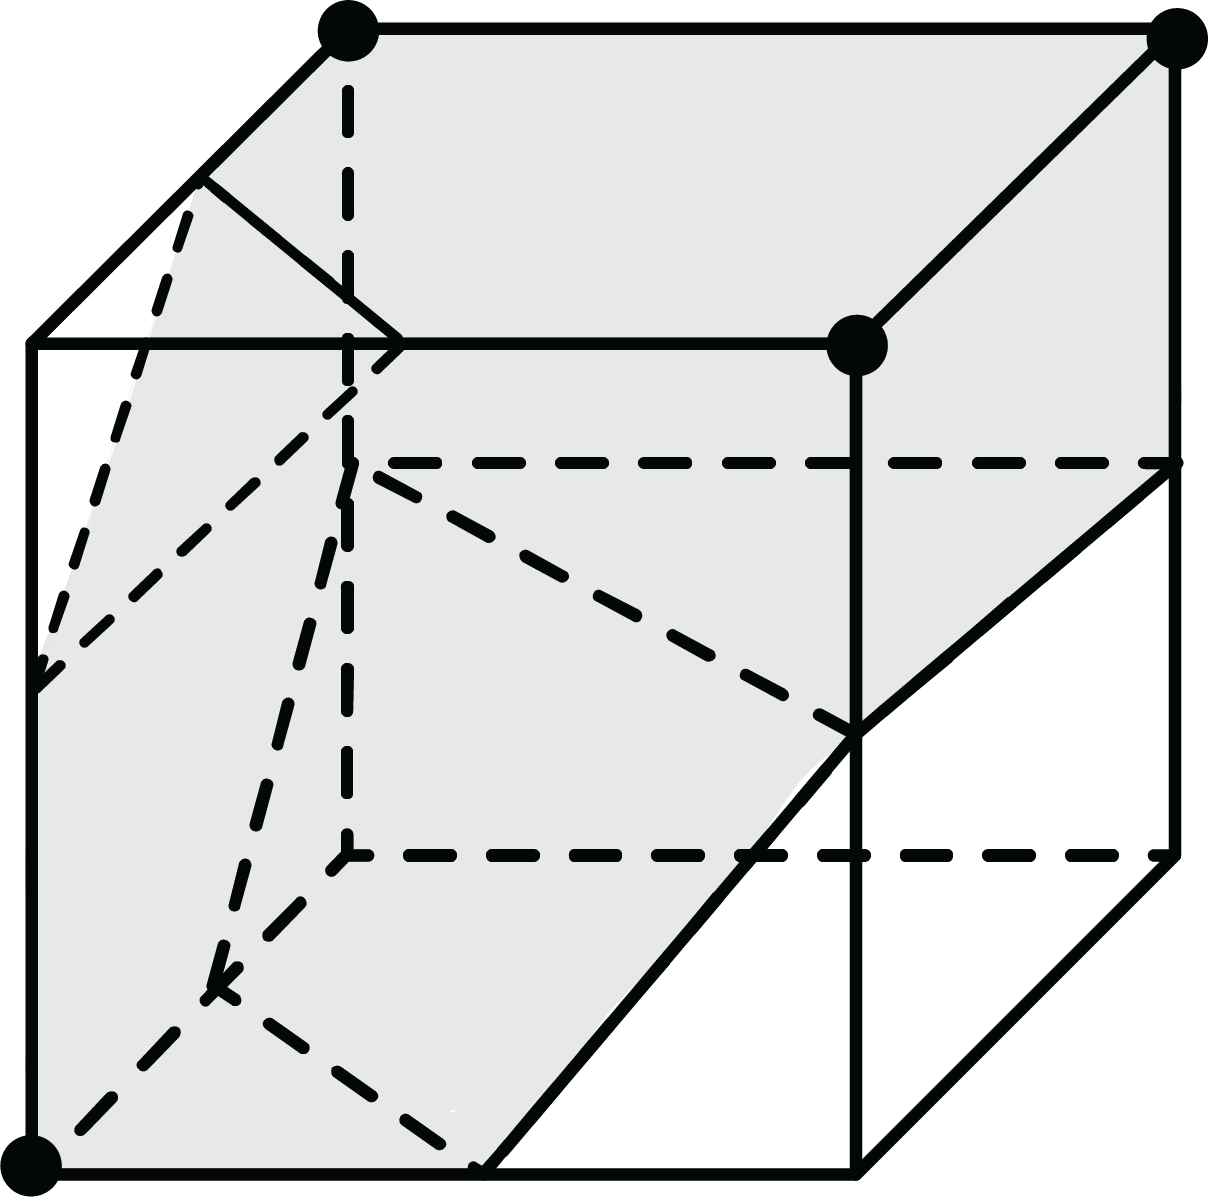
\includegraphics[width=1cm]{Figures/case 28.png} & $\frac{5}{144}$ \\

        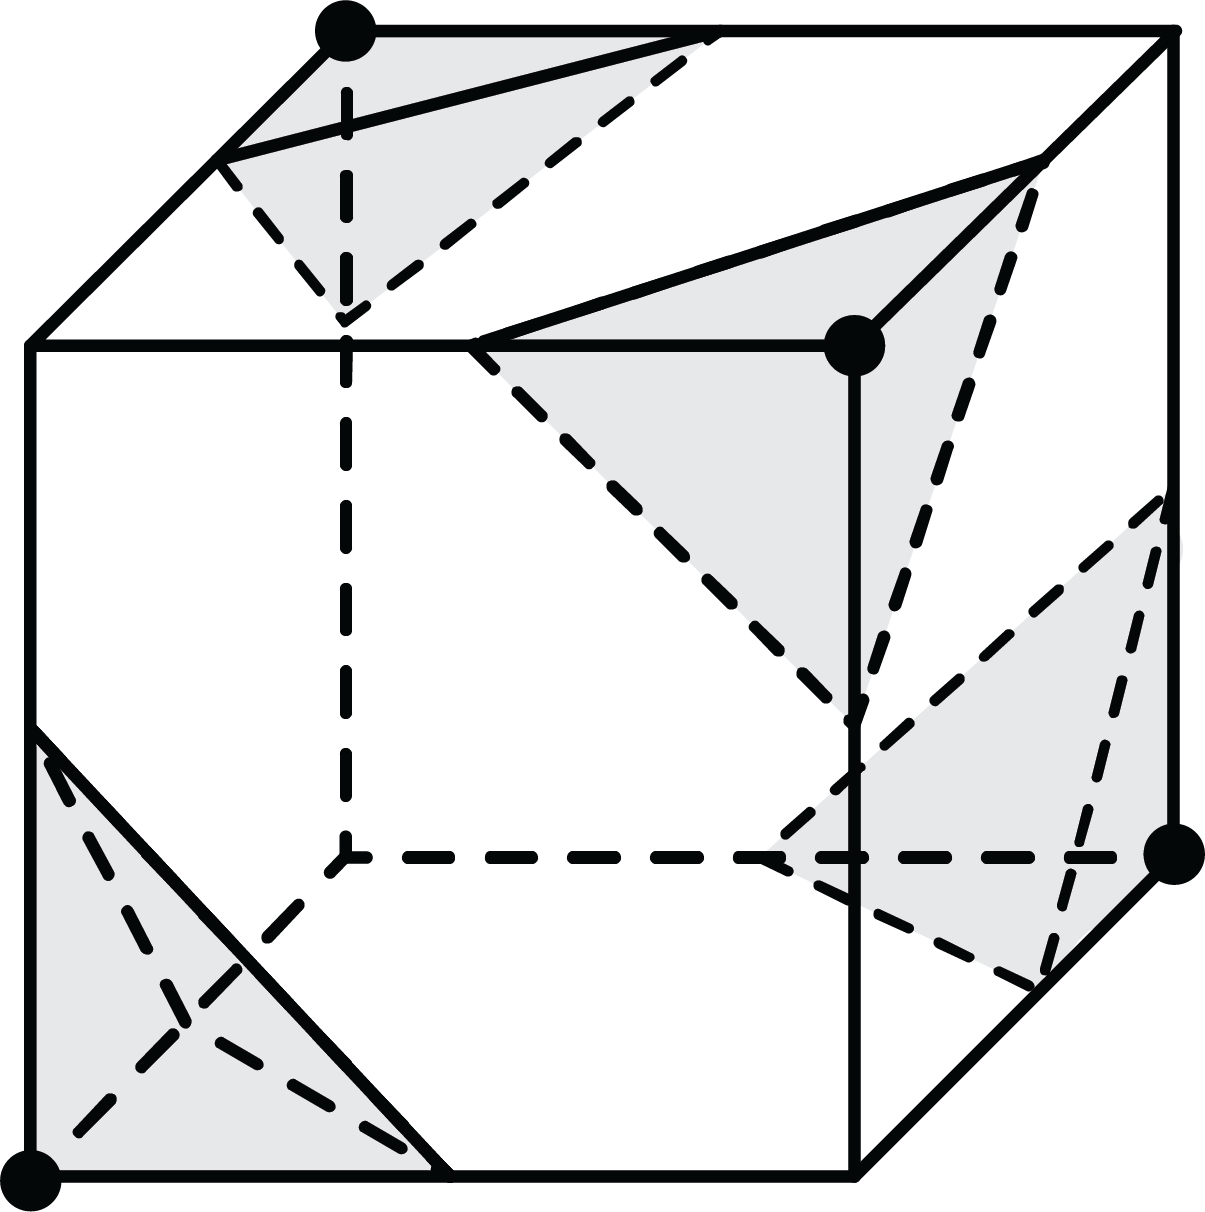
\includegraphics[width=1cm]{Figures/case 14.png} & $4 \times \frac{1}{48}$ & 4 tetrahedrons & $\frac{1}{12}$ & 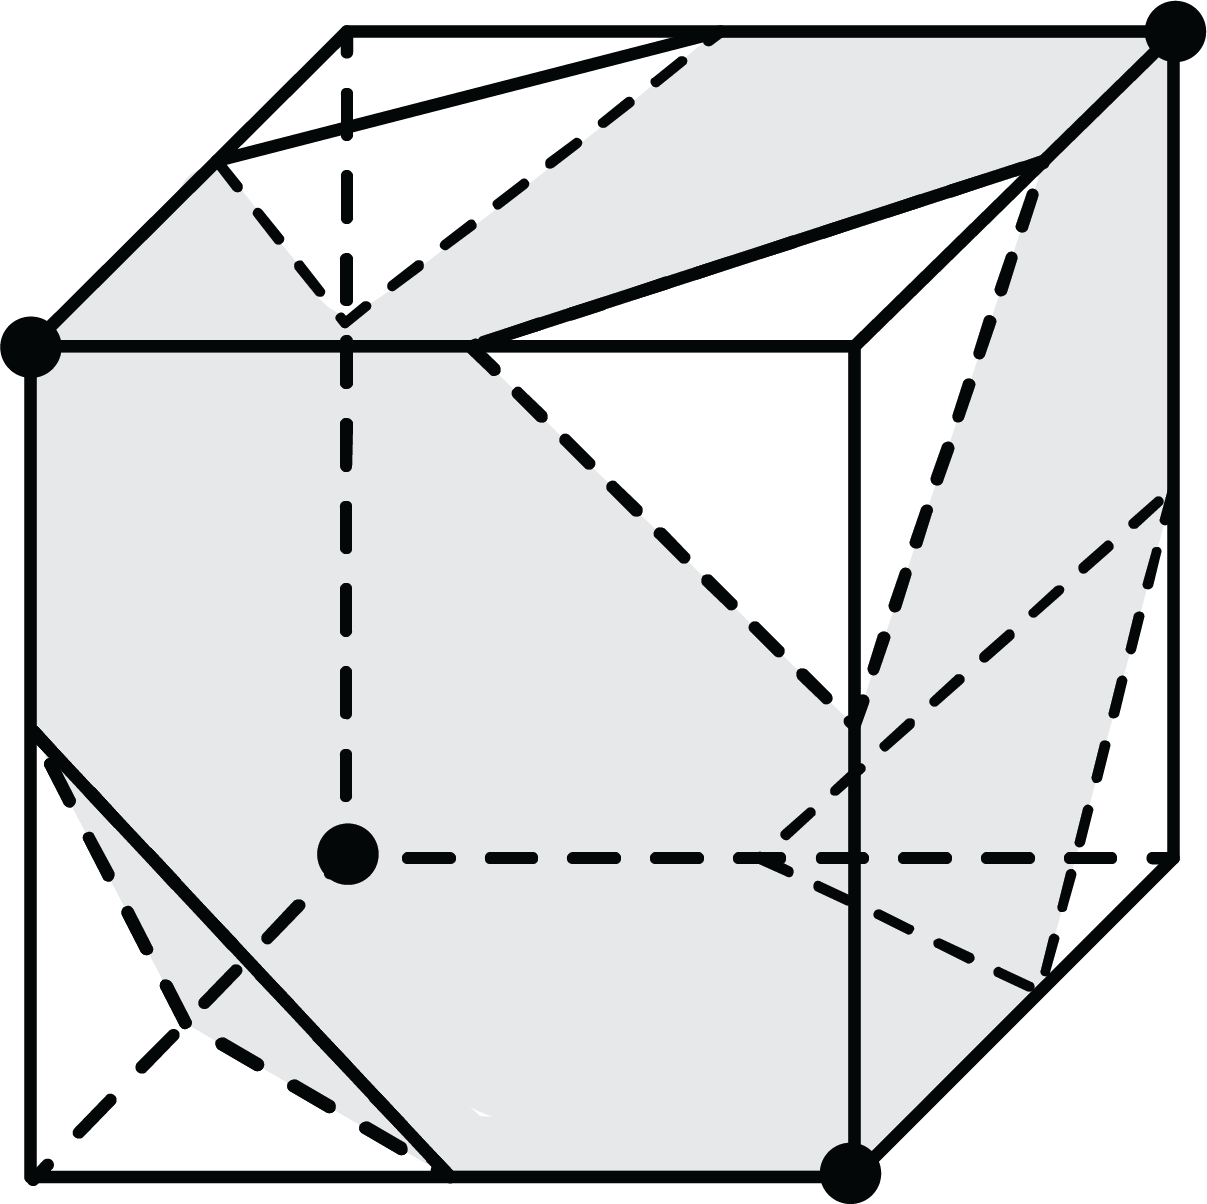
\includegraphics[width=1cm]{Figures/case 29.png} & $\frac{11}{12}$\\

        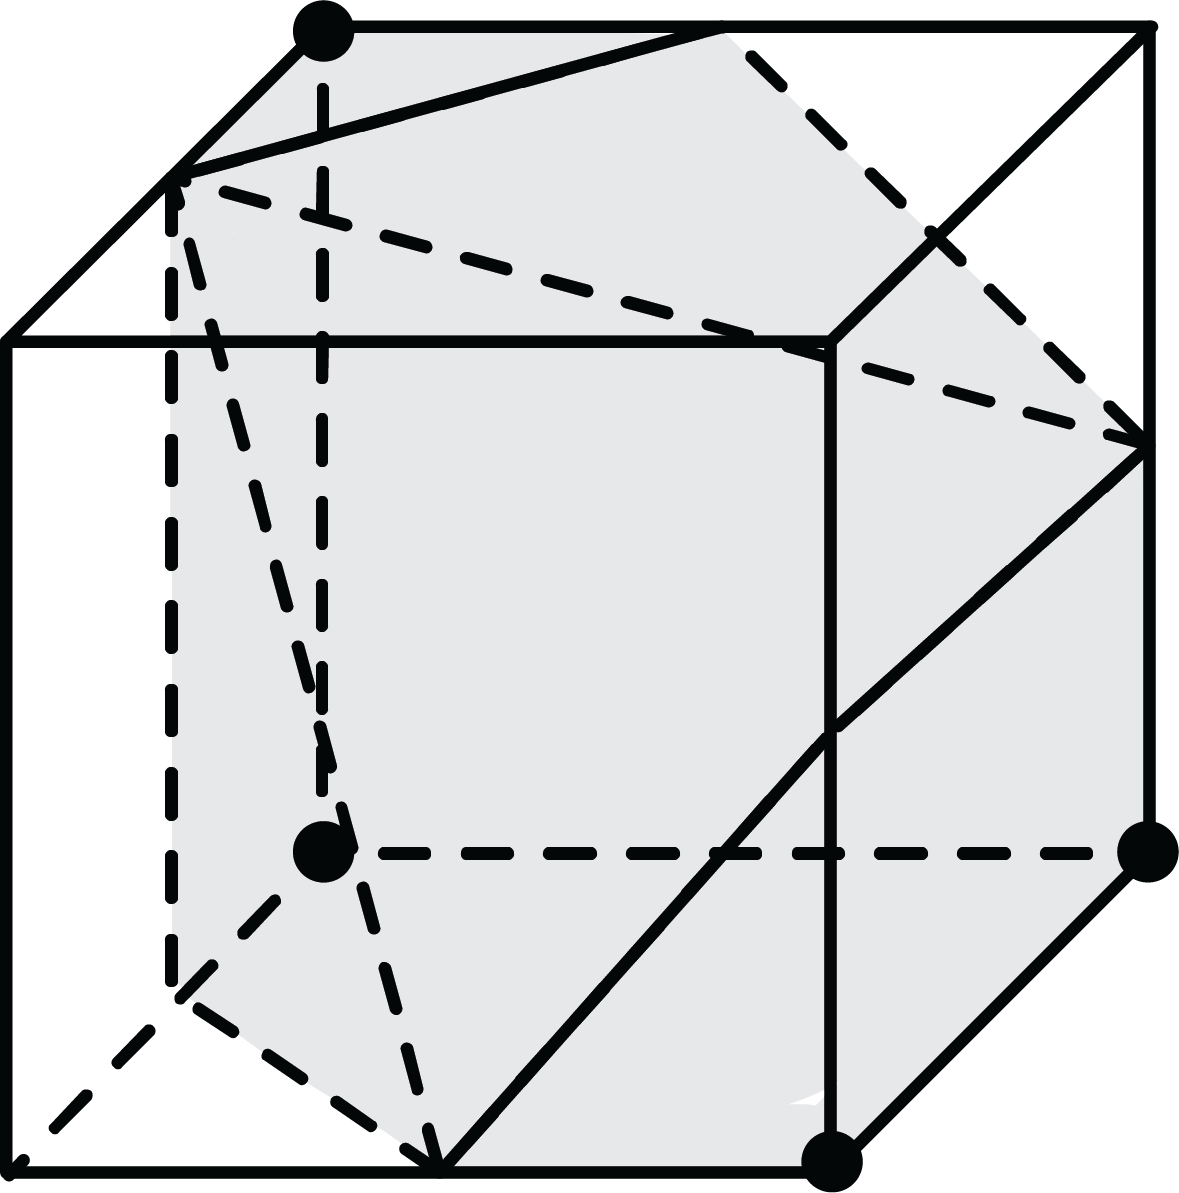
\includegraphics[width=1cm]{Figures/case 15.png} & $\frac{1}{8} \times 3 + \frac{1}{24}$ &2 prisms, 2 tetrahedrons& $\frac{5}{12}$ & 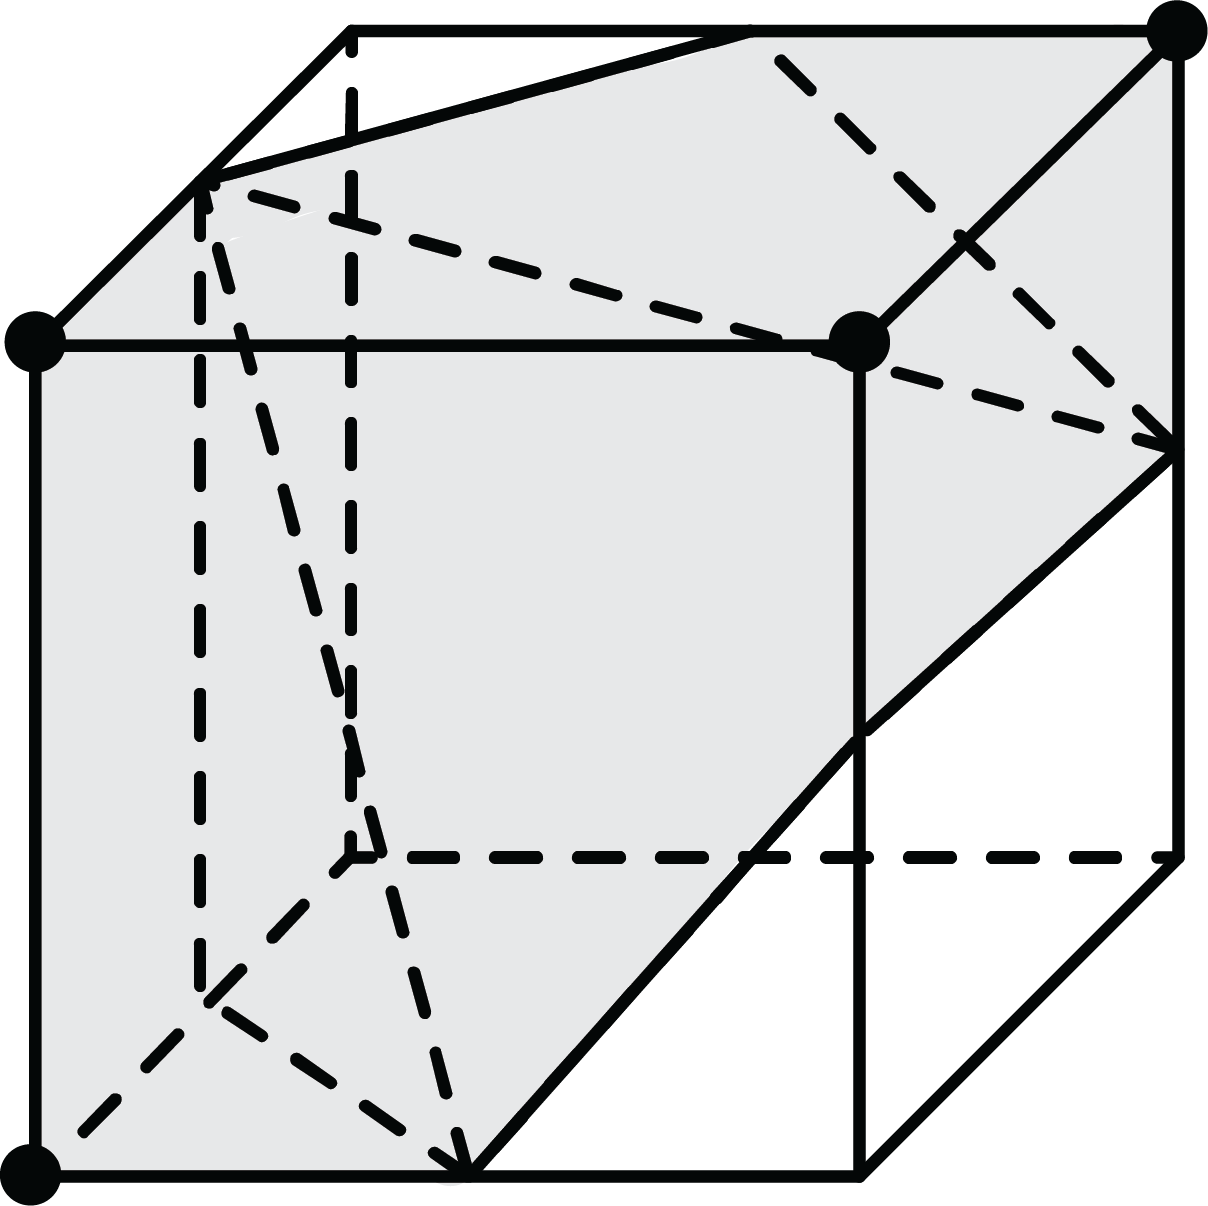
\includegraphics[width=1cm]{Figures/case 30.png} & $\frac{7}{12}$ \\
        
    \end{tabular}
    \caption{Volume of 3D model within a cube specification for 30 cases (15 configurations)}
    \label{tab:volume configurations}
\end{table}

\begin{multicols}{2}

However the Marching Cube method proposed by \cite{loren} has limitations. The algorithm can lead to cracks because the same configuration can be tiled in different ways \cite{lewiner}. Lewiner optimized the algorithm by considering more cases (32 base cases instead of 15). However, in our research scope, we only speculate the volume based on Lorensen's lookup table to estimate the practicability of our assumption before further improvement with Lewiner's extended one.

The vertex with bold black dot is the false one, which means this vertex possesses value below the threshold level and is totally inside the 3D reconstructed polygonal mesh. The volume of the model within each cube need considering is highlighted from the initial 15 base cases to next 15 reversed cases with calculation formulas, explanation, and results provided simultaneously. Specially, in the last 5 cases (four False vertices and four True vertices), although not only the topological mesh configuration but also the vertices relative position remain unchanged while being reversed, the intrinsic volume essentially changes. Therefore when speculating volume configurations for $256$ cases (for fast query), we use the $\text{vertex}_0 (x,y,z)$ as pivot to classify case $26,27,28,29,30$ from case $11,12,13,14,15$.

Considering implementation, supposing the volumetric data named is specified in size $(N,M,P)$, we initialize a 3D array named $\text{Cube}$ of size $(N-1, M-1, P-1)$. We take the $\text{vertex}_0 (x,y,z)$ as pivot to manage the whole cube or $7$ last other vertices $(x+1, y,z), \dots, (x+1,y+1,z+1)$. Therefore, $\text{Cube}[i,j,k] = \text{VolumeLookup}(i,j,k)$ with $i \leq N-1, j \leq M-1, k \leq P-1$ and $\text{VolumeLookup}$ returns the volume based on above 30 cases.

Finally, we can sum up all the value in this 3D array to get the total volume of our 3D object. However, this way of storing calculation results is not suitable when updates (e.g slicing, mesh edition) occur. The time complexity is $O(Q \times N \times M \times P)$ with $Q$ is the number of update events.

\subsection{Binary indexed tree}
The Binary indexed tree (BIT), also Fenwick Tree, is a widely used data structure in competitive programming, introduced in the research paper "A new data structure for cumulative frequency tables" by Peter M. Fenwick \cite{fenwick}. The BIT exhibits the following characteristics: querying the result of a subproblem in $O(logN)$, updating the value for one element in $O(logN)$, or a segment in $O(NlogN)$, low memory usage $O(N)$, and fast processing speed (due to bitwise operations). In detail, with each update operation, the last bit is always shifted up at least 1 time, leading to the maximum of $logN$ times of bit shifts.

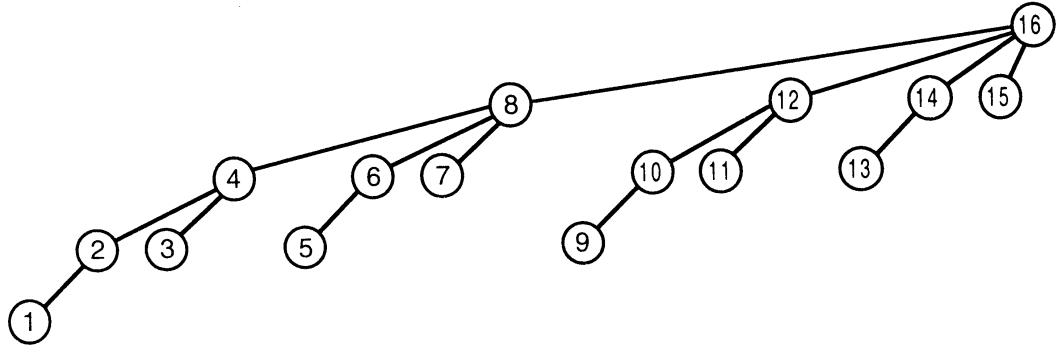
\includegraphics[width=0.45\textwidth]{Figures/Fenwick Tree.png}
\textbf{Figure 4:} The updating binary indexed tree \cite{fenwick} \\

In BIT, the element $i_{th}$ stores the result $F[i]$ of the subproblem containing $2^k$ elements starting/ending at position $i$, where $k$ is the lowest set bit in the binary representation of $i$. Observing the representation of the tree above, we can easily see that nodes with odd indices manage only themselves, while nodes with index $id$ will have a parent with index $id + 2^k$. Finding the value of $2^k$ is simply done by performing the bitwise operation: $2^k = -id \& id$.


\subsubsection{3D Binary indexed tree}

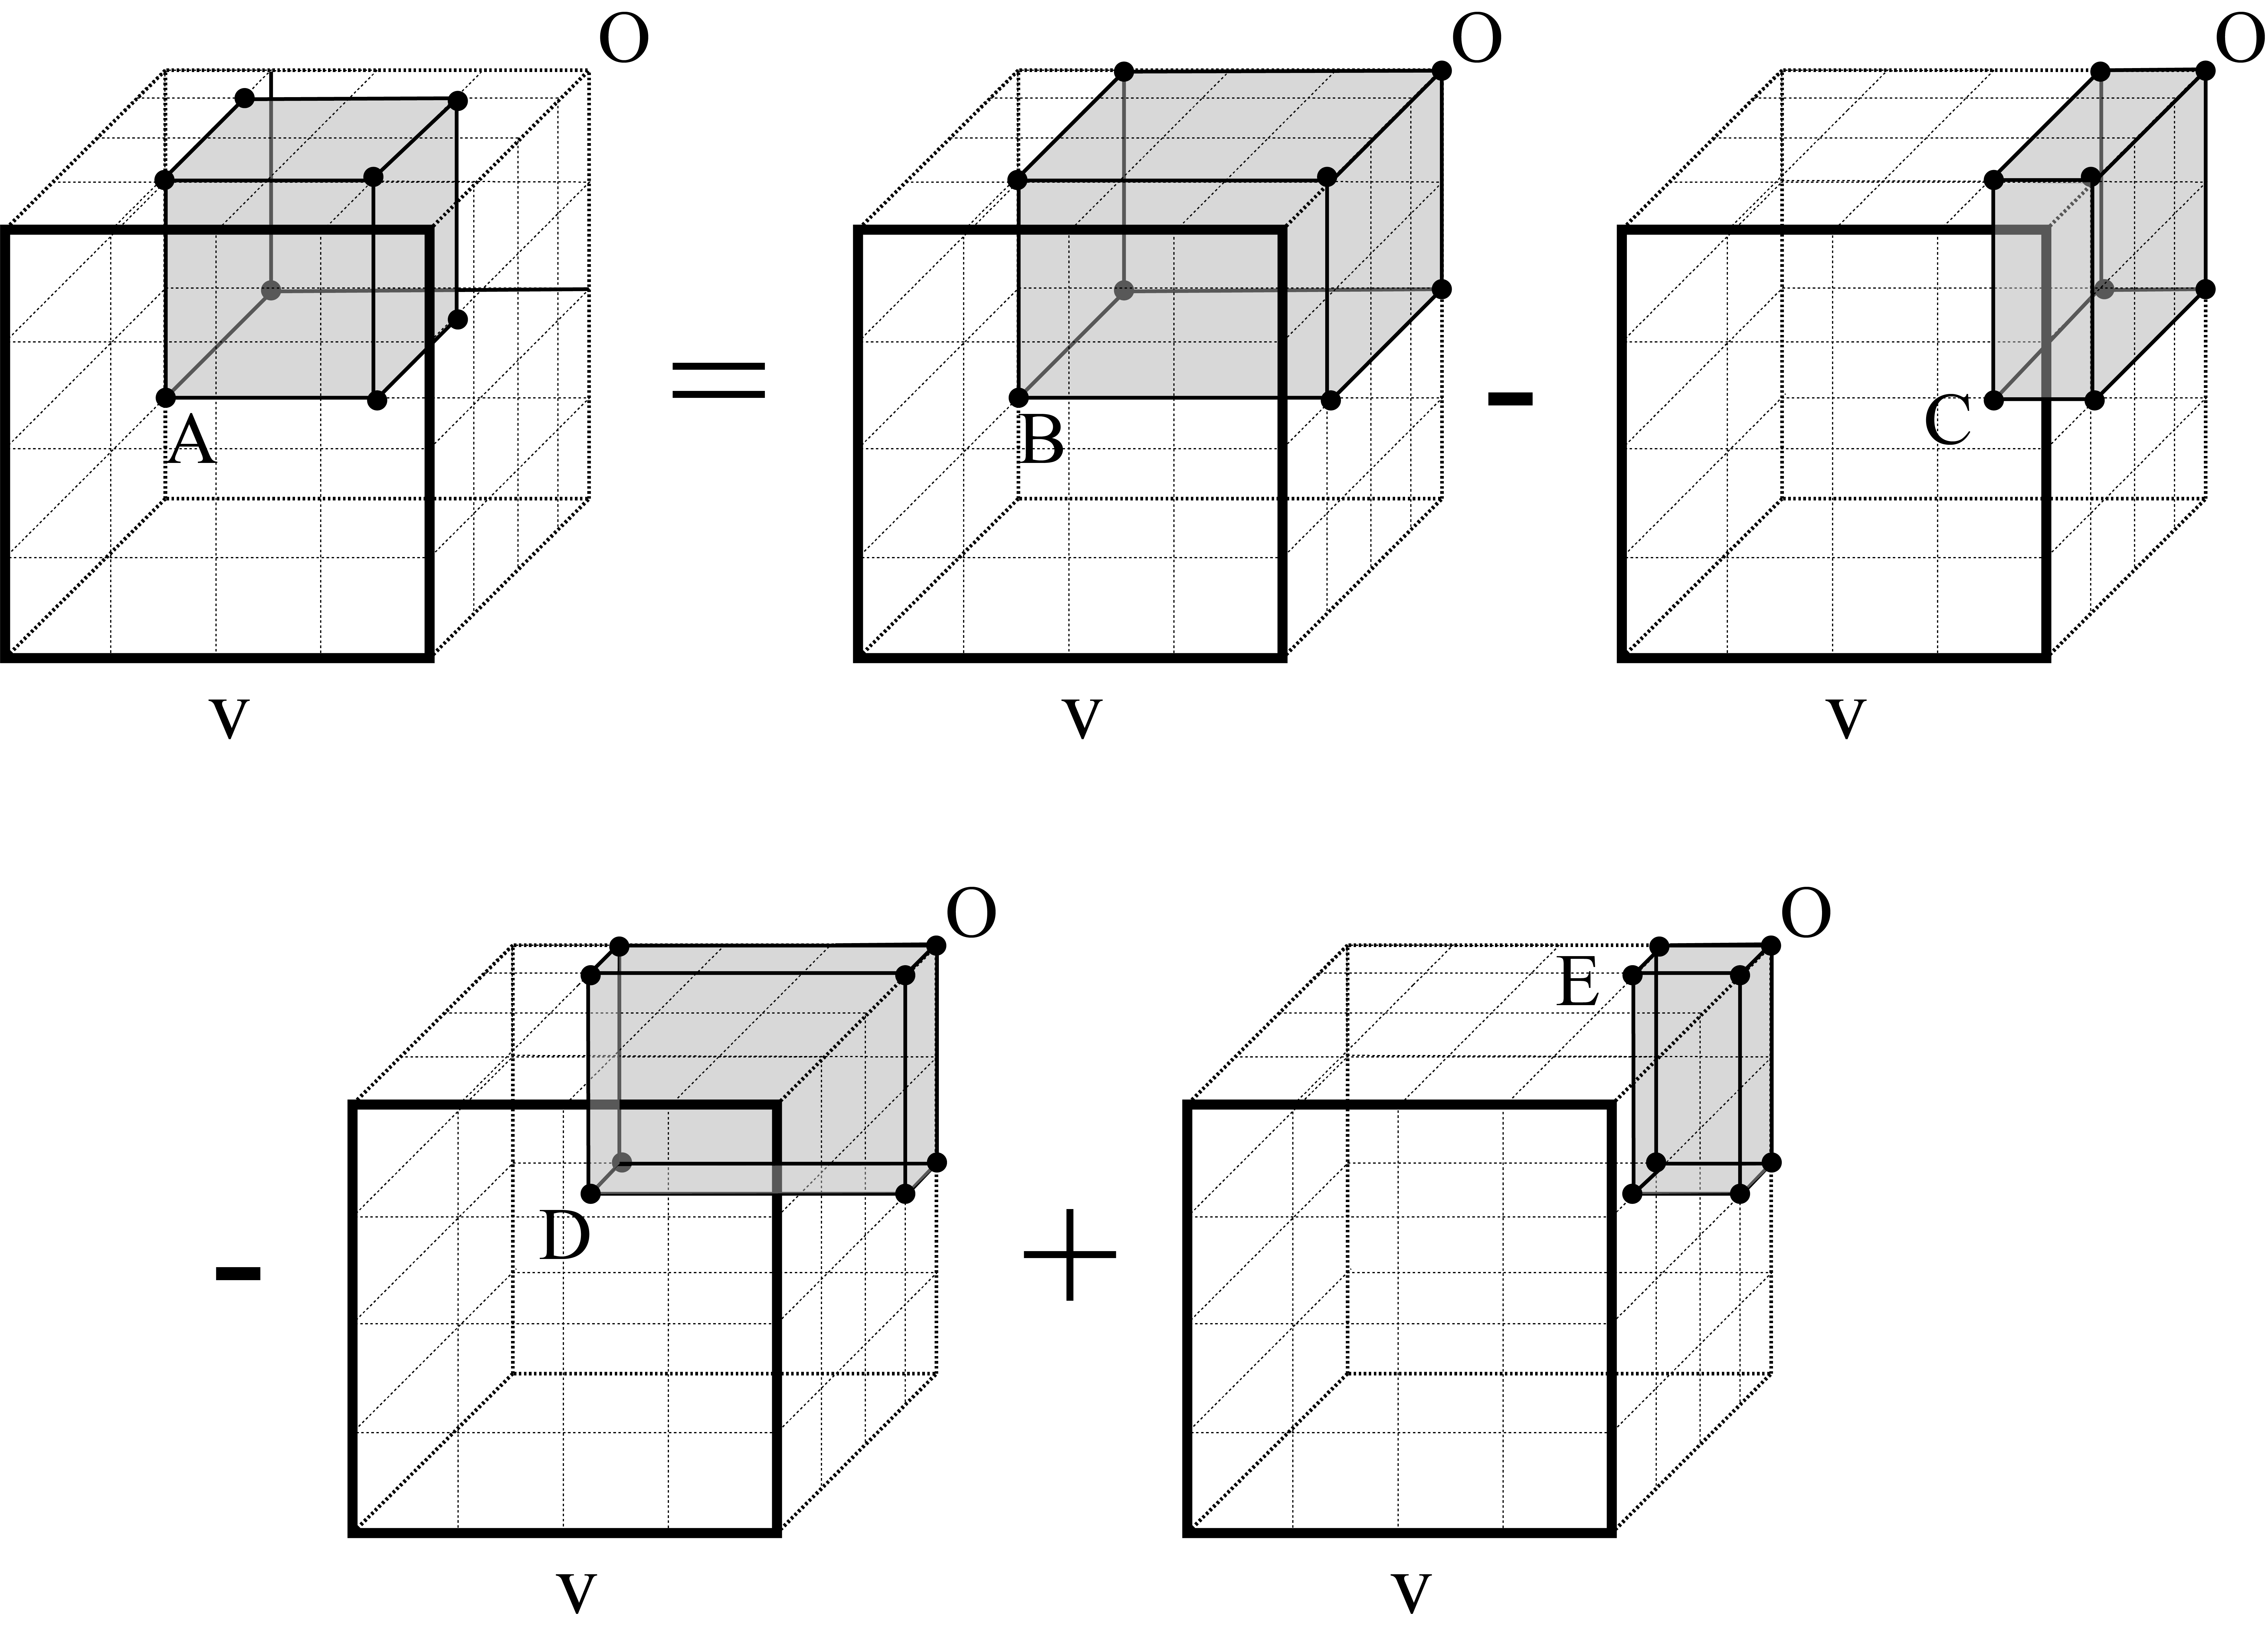
\includegraphics[width=0.47\textwidth]{Figures/3D BIT.png}
\textbf{Figure 5:} Query a region in 3D BIT \\

This is a novel application of binary indexed trees into three-dimensional arrays. We employ the principle of inclusion and exclusion to query the sum of elements over a 3D space by excluding surrounding parts, similar to slicing but without data loss). We can perform updates on a 3D space (altering the mesh reconstruction) with minimal complexity of $O(logN \times logM \times logP)$, where $(N, M, P)$ represent the dimensions of volumetric data. The formula of 3D query is:

$$ \text{Q}(x1, y1, z1, x2, y2, z2) = \text{S}(x2, y2, z2) $$
$$ - \text{S}(x2, y2, z1 - 1) - \text{S}(x2, y1 - 1, z2) $$
$$ + \text{S}(x2, y1 - 1, z1 - 1) - \text{S}(x1 - 1, y2, z2) $$
$$ + \text{S}(x1 - 1, y2, z1 - 1) + \text{S}(x1 - 1, y1 - 1, z2) $$
$$ - \text{S}(x1 - 1, y1 - 1, z1 - 1) $$

$Q$, $S$ represent the $\text{QueryByRegion}$ and $\text{getSum}$ function respectively in the implementation code. In the marching cubes three loop, instead of storing data into 3D array $\text{Cube}$, we build cumulatively the BIT by calling $\text{update}$ function as $BIT[i,j,k] = update(i,j,k,value)$ with $value$ is the $\text{VolumeLookup}(i,j,k)$.

You can find the open-source code published online on Github in the Open Source section.

\section{Experiments}
\subsection{Setup experiments}
We experimented our algorithm both on simple shape (sphere) with predetermined radius and complex 3D structure (cardiac model) with predetermined volume. The computed volume and labelled volume is represented in table 2. Also, we compare the time processing of BIT query with bruteforce method. Each case is computed 5 times to ensure consistency. In medical imaging, especially dealing with volumetric data acquired from CT, MR. We have to consider the pixel spacing value, slick thickness for accurate unit conversion from pixel/voxel world into real world unit ($\text{mm}^3$ or $\text{ml}$). We run the algorithm only with CPU. 

\begin{table*}[]
    \centering
    \begin{tabular}{c|c|c|c|c|c}
    
    \midrule
    \textbf{Shape} & \textbf{Radius} & \textbf{BIT time ($s$)} & \textbf{BF time ($s$)} & \textbf{Cal V ($\text{cm}^3$)} & \textbf{La V ($\text{cm}^3$)} \\ 
    \midrule
    $50 \times 50 \times 50$ & $10$ & $0.0$ & $0.026$ & $2.573$ & $2.645$ \\ 
    & $15$ & $0.0$ & $0.016$ & $8.546$ & $8.929$ \\ 
    & $20$ & $0.0$ & $0.015$ & $20.079$ & $21.166$ \\ 
    & $25$ & $0.0$ & $0.020$ & $39.120$ & $41.340$ \\ 
    \midrule
    $100 \times 100 \times 100$ & $20$ & $0.0$ & $0.151$ & $20.668$ & $21.166$ \\ 
    & $25$ & $0.0$ & $0.154$ & $8.546$ & $41.340$ \\ 
    & $30$ & $0.0$ & $0.168$ & $69.535$ & $71.435$ \\ 
    & $35$ & $0.0$ & $0.155$ & $110.428$ & $113.436$ \\ 
    \midrule
    $250 \times 250 \times 250$ & $20$ & $0.0$ & $2.284$ & $71.195$ & $71.435$ \\ 
    & $25$ & $0.0$ & $2.174$ & $112.879$ & $113.436$ \\ 
    & $30$ & $0.0$ & $2.295$ & $168.133$ & $169.328$ \\ 
    & $35$ & $0.0$ & $2.224$ & $239.140$ & $241.094$ \\ 
    \midrule
    $500 \times 500 \times 500$ & $20$ & $0.0$ & $19.962$ & $21.197$ & $21.166$ \\ 
    & $25$ & $0.0$ & $19.193$ & $71.408$ & $71.435$ \\ 
    & $30$ & $0.0$ & $18.946$ & $169.2042$ & $169.328$ \\ 
    & $35$ & $0.0$ & $19.714$ & $240.021$ & $241.094$ \\ 

    \end{tabular}
    \caption{Experiment on sphere}
    \label{tab:Experiment sphere display}
\end{table*}

\begin{table*}[]
    \centering
    \begin{tabular}{c|c|c|c|c|c}
    
    \midrule
    \textbf{Structure} & \textbf{Shape} & \textbf{Processing time ($s$)} & \textbf{Cal V ($\text{ml}$)} & \textbf{La V ($\text{ml}$)} \\ 
    \midrule
    Left ventricle & $512 \times 600 \times 600$ & 127.960 & 120.06618 & 100-140 \\
    Right ventricle & $512 \times 600 \times 600$ & 126.965 & 75.08047 & 50-100 \\
    Left atrium & $512 \times 600 \times 600$ & 103.747 & 30.93378  & 25-35 \\
    Right atrium & $512 \times 600 \times 600$ & 102.356 & 100.00465 & 80-110 \\
    Myocardium & $512 \times 600 \times 600$ &108.042 & 183.84389 & \\
    Ascending arota & $512 \times 600 \times 600$ & 204.393 & 25.047446 & 20-30  \\
    Descending aorta & $512 \times 600 \times 600$ & 275.57 & 125.333 & 100-150 \\
    Pulmonary trunk & $512 \times 600 \times 600$ & 244.903 & 26.249936 & 20-30  \\
    Vena cava & $512 \times 600 \times 600$ & 169.776 & 107.07984  & \\
    Auricle & $512 \times 600 \times 600$ & 175.576 & 12.508784 & 10-15 \\
    Coronary Artery & $512 \times 600 \times 600$ & 114.604 & 13.09273  & \\

    \end{tabular}
    \caption{Experiment on cardiac volumetric data}
    \label{tab:Experiment cardiac display}
\end{table*}


\subsection{Results and evaluation}
Observing the table 2, the Brute Force (BF) time increases correspondingly wih the size of volumetric data. However, by query the BIT tree with Cython implementation, the time of query of any part is only $0.0$. You can find the open-source code and run yourself to reconfirm. The more high-resolution the volumetric data is, the more accurate of calculated volume we can approximate. Meanwhile, with medical volumetric data (cardiac structures), the Processing time represents both time dedicated to Marching Cubes and BIT initialization. Our Marching cubes implementation is basic, enlongering the processing time.  
 
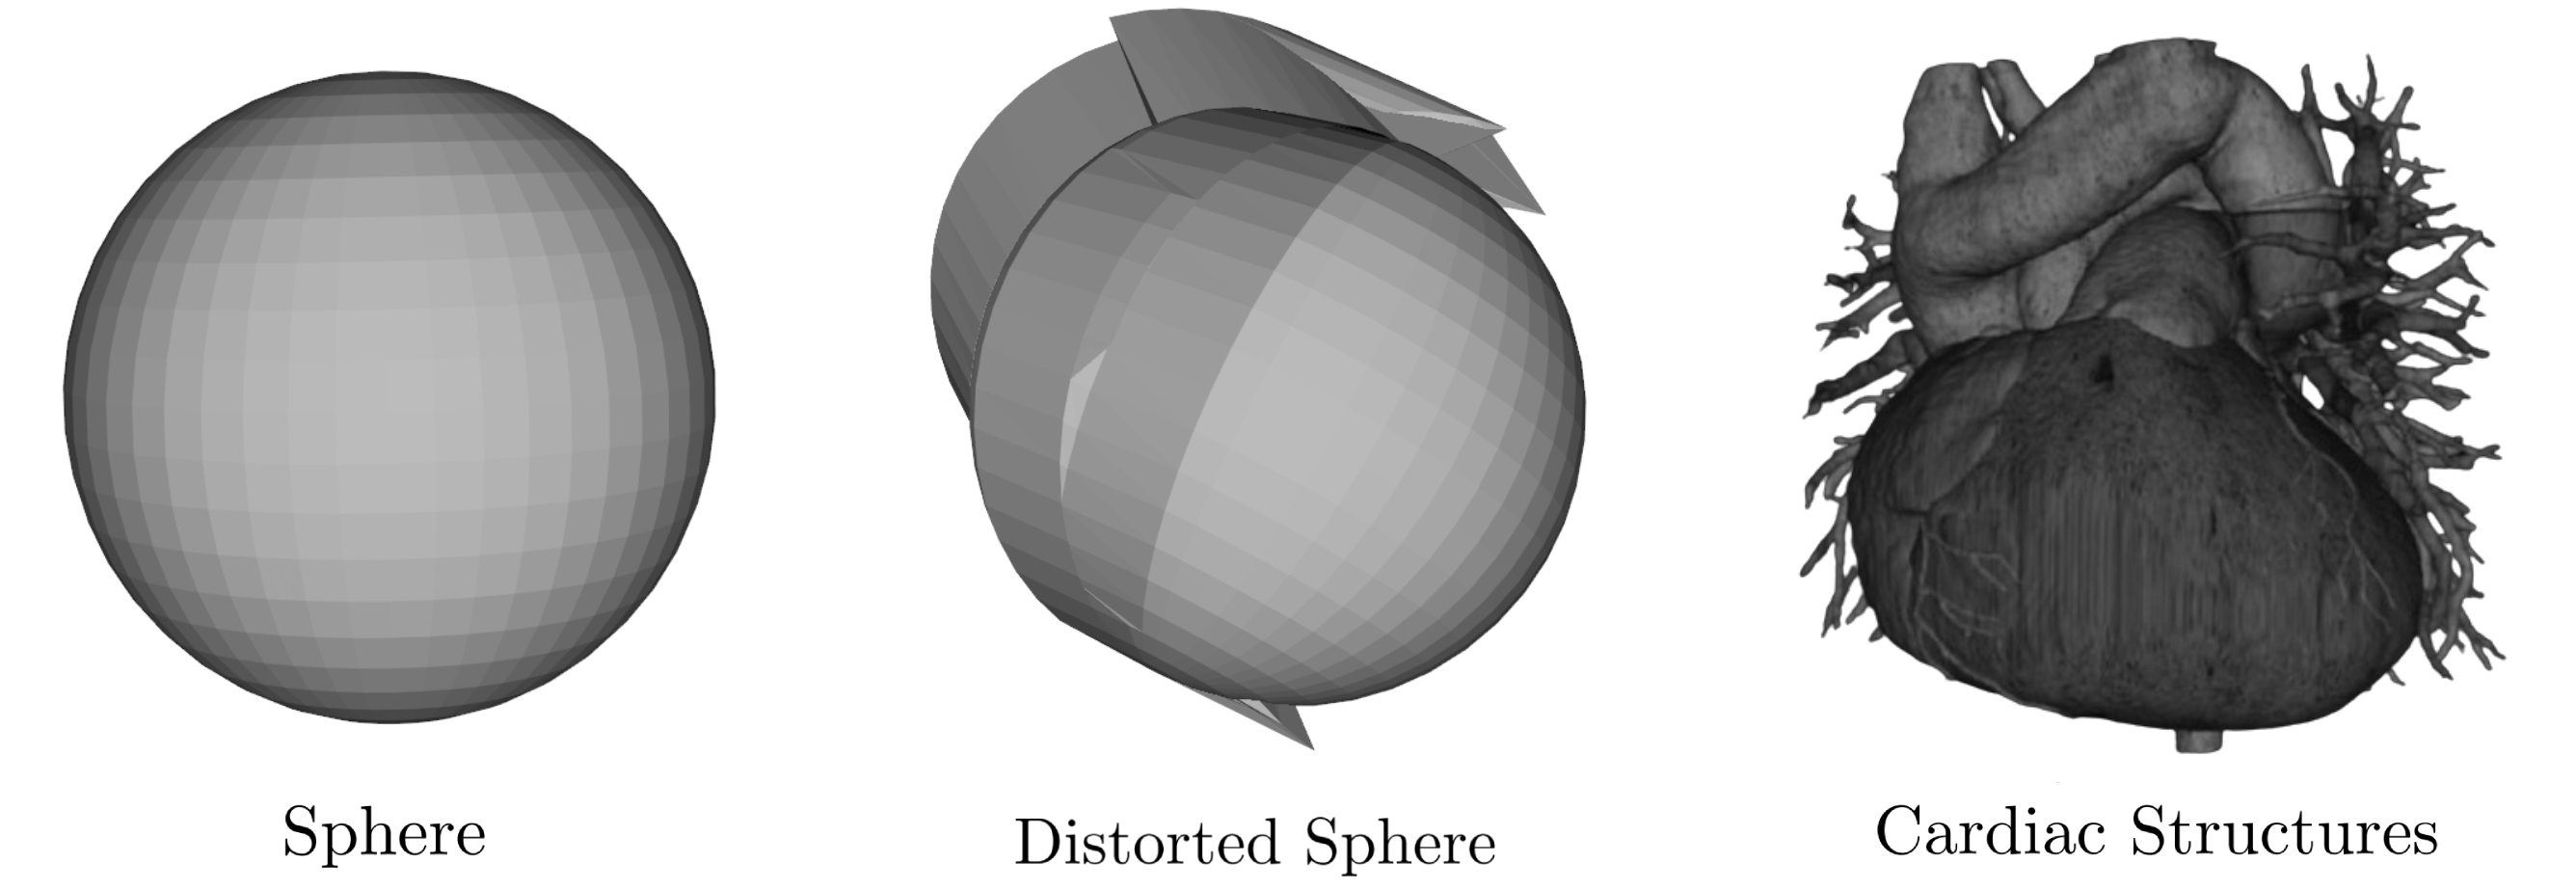
\includegraphics[width=0.45\textwidth]{Figures/Experiment.png}
\textbf{Figure 6:} Experiment on distorted mesh and cardiac structures \\

We developed a software called Vascular \cite{vascular} that can distort and slice the mesh. Then we use our BIT data structure to estimate the new volume of 3D volumetric data with time-efficiency in real time.  

\section{Open Source}
We implemented the Marching Cubes algorithm based on Lorensen's lookup table instead of Lewiner's. We initialized two lookup table volume configurations named $\text{VOLUME\_CASE\_LOOKUP}$ of size $30$ and $\text{VOLUME\_LOOKUP}$ of size $256$. We implemented the code with Cython, an efficient Python to C compiler, to optimize performance. This approach allowed us to efficiently handle the volume rendering process, ensuring accurate results while maintaining computational efficiency. We also published the pure Python code of the algorithm. However, the pure Python code should only be used for small-sized 3D arrays. For medical volumetric data, especially high-resolution ones, it's recommended to utilize the C/C++ implementation or use Cython.

Code link: https://github.com/VISEF-ISEF-team/Volume-Computation-of-3D-Reconstructed-Models-from-Volumetric-Data-using-Binary-Indexed-Tree.git

\newpage
\bibliographystyle{IEEEtran}
\bibliography{references}
\end{multicols}
\end{document}
